\documentclass[a4paper,11pt,twoside,onecolumn,final,openright]{book}
\usepackage[doublespace,indent]{thesisdavid}
\usepackage[latin1]{inputenc}
\usepackage{subfigure}
\usepackage[english]{babel}
\usepackage{url}
\usepackage{epsfig}
\usepackage{epstopdf}
\usepackage{makeidx}
\usepackage{multirow}
\usepackage{indentfirst}
\usepackage[font=normalsize]{caption}
\usepackage{colortbl}
\usepackage{adjustbox}
\usepackage{enumitem}

\usepackage{array,booktabs,arydshln}
\usepackage{rotating}
\usepackage{hyphenat}
\usepackage{graphicx}
\usepackage{xspace}
\usepackage{stfloats}
\usepackage{flushend}
\usepackage{listings}
\usepackage{color}

\definecolor{gray}{rgb}{0.4,0.4,0.4}
\definecolor{darkblue}{rgb}{0.0,0.0,0.6}
\definecolor{cyan}{rgb}{0.0,0.6,0.6}

\lstset{
  basicstyle=\ttfamily,
  columns=fullflexible,
  showstringspaces=false,
  commentstyle=\color{gray}\upshape
}

\definecolor{dkgreen}{rgb}{0,0.6,0}
\definecolor{gray}{rgb}{0.5,0.5,0.5}
\definecolor{mauve}{rgb}{0.58,0,0.82}
\lstset{frame=tb,
  language=Java,
  aboveskip=3mm,
  belowskip=3mm,
  showstringspaces=false,
  columns=flexible,
  basicstyle={\small\ttfamily},
  numbers=none,
  numberstyle=\tiny\color{gray},
  keywordstyle=\color{blue},
  commentstyle=\color{dkgreen},
  stringstyle=\color{mauve},
  breaklines=true,
  breakatwhitespace=true,
  tabsize=3
}

\lstdefinelanguage{XML}
{
  morestring=[b]",
  morestring=[s]{>}{<},
  morecomment=[s]{<?}{?>},
  stringstyle=\color{black},
  identifierstyle=\color{darkblue},
  keywordstyle=\color{cyan},
  morekeywords={xmlns,version,type}% list your attributes here
}

\newcolumntype{M}[1]{>{\centering\arraybackslash}m{#1}}

\newcommand{\red}[1]{\textcolor{red}{#1}}
\newcommand{\todo}[1]{\textcolor{red}{\{TODO:} #1\textcolor{red}\}}

\definecolor{light}{gray}{.85}

\begin{document}

% Initial pages.


\def\date{October 2015}
\def\titulo{SleeveAR: Augmented Reality for Rehabilitation Using Realtime Feedback}
\def\avitima{Jo\~{a}o Tiago Proen\c{c}a F\'elix Vieira}

\thispagestyle{empty}

\begin{singlespace}
\vbox to\textheight{%
%--------------------------------------------------
\vskip-1.3in%---------- LOGO E NOME IST/UTL -------
%--------------------------------------------------
\hskip-17mm\vbox to50mm{
\vfil
\begin{tabular}{l}

\includegraphics[width=9cm]{imgs/Logo_IST_web.pdf}
\end{tabular}
\vfil
\vfil
}%
%--------------------------------------------------
\vskip6mm%---------- TTULO -----------------------
%--------------------------------------------------
\vbox to25mm{\LARGE\bf
\vfil
\begin{center}
\titulo
\end{center}
\vfil
}%
%--------------------------------------------------
\vskip10mm%---------- NOME E GRAU ACTUAL -----------
%--------------------------------------------------
\vbox to25mm{\large
\vfil
\begin{center}
{\Large\bf \avitima}\\   % author's name
\end{center}
\vfil
}%
%--------------------------------------------------
\vskip10mm%---------- GRAU A OBTER -----------------

%--------------------------------------------------
\vbox to8mm{\large
\vfil
\centerline{Dissertation for the Degree of Master of}
%\vskip6mm
\centerline{Engineering Systems and Computer Engineering}
\vfil
}%
% %--------------------------------------------------
\vskip10mm %---------- JURI -------------------------
% %--------------------------------------------------
\vbox to7mm{\bf
\vfil
\begin{center}
{\bf Jury}\\
\end{center}
\vfil
}%

\vbox to28mm{
\vfil
{\small
\begin{center}
\begin{tabular}{p{0.2\textwidth}l}
President: &  PERGUNTAR AO ORIENTADOR \\
Advisor: & Prof. Joaquim Jorge\\
Co-Advisor: & Prof. Artur Ars\'enio\\
Member: & PERGUNTAR AO ORIENTADOR \\
\end{tabular}
\end{center}
}
\vfil
}%
%--------------------------------------------------
\vskip28mm%---------- DATA -------------------------
%--------------------------------------------------
\vbox to4mm{\Large\bf
\vfil
\begin{center}
\date
\end{center}
\vfil
}%
%--------------------------------------------------
}%vbox
\end{singlespace}
\newpage

\chapter*{Acknowledgements}
%\chapter*{Acknowledgements}
\thispagestyle{empty}

I would like to thank my canary.
Ana Paula Morais Cabral fisioterapeuta


\vfill
\begin{flushright}
  \begin{minipage}{8cm}
    \begin{center}
      Lisboa, \date

      \avitima
    \end{center}
  \end{minipage}
\end{flushright}

\cleardoublepage

  %%%%%%%%%%%%%%%%%%%%%%%%%%%%%%%%%%%%%%%%%%%%%%%%%%%%%%%%%%%%%%%%%%%%%%%%%%%%%
  %
%%%%%                            DEDICATORIAS
 %%%
  %

\chapter*{}
\thispagestyle{empty}

% DEDICAR!
\vfill
\mbox{}
\vfill\Large
\begin{flushright}
  \begin{minipage}{8cm}
    \begin{center}

For blablablablabla,\\

    \end{center}
  \end{minipage}
\end{flushright}
\normalsize\vfill

\cleardoublepage

  %%%%%%%%%%%%%%%%%%%%%%%%%%%%%%%%%%%%%%%%%%%%%%%%%%%%%%%%%%%%%%%%%%%%%%%%%%%%%
  %
%%%%%                                RESUMO
 %%%
  %

\chapter*{Resumo}
\thispagestyle{empty}
 
My abstract in Portuguese.

\newpage

  %%%%%%%%%%%%%%%%%%%%%%%%%%%%%%%%%%%%%%%%%%%%%%%%%%%%%%%%%%%%%%%%%%%%%%%%%%%%%
  %
%%%%%                            ABSTRACT
 %%%
  %

\chapter*{Abstract}
\thispagestyle{empty}

After being exempted from in-clinic physical therapy, 
	it is usual for a patient to continue performing exercises 
	outside of the clinic and without any therapist's supervision.
	While performing unsupervised exercises, it would be desirable 
	to receive similar feedback as the one provided by a physical therapist, to maintain 
	a certain quality in the task execution.
	To address this problem, several approaches using feedback for rehabilitation have been implemented. Unfortunately, the test subjects frequently reported difficulty in completely understanding the feedback given to them, therefore failing to correctly execute the given movement.

\newpage


\chapter*{Palavras Chave \\ Keywords}
\thispagestyle{empty}

\section*{Palavras Chave}
{\large % EM PORTUGUES

\noindent xxx

\noindent xxx

\noindent xxx

\noindent xxx

\noindent xxx

}

\section*{Keywords}

{\large % EM INGLES

\noindent xxx

\noindent xxx

\noindent xxx

\noindent xxx

\noindent xxx

}

\vfill


\cleardoublepage

\pagestyle{plain}
\pagenumbering{roman}

 
\def\contentsname{Contents}
\tableofcontents
\newpage

\listoffigures
\newpage

\listoftables

\cleardoublepage

       


\chapter*{Acronyms}

\begin{singlespace}

\begin{acronym}
	\acro{AR}{Augmented Reality}
	\acro{PT}{Physical Therapist}
	\acro{RS}{Rehabilitation System}
	\acro{KP}{Knowledge of Performance}
	\acro{KR}{Knowledge of Results}
	\acro{MFM}{Multimodal Feedback Manager}
	\acro{DTW}{Dynamic Time Warping}
	\acro{FS}{Feedback Service}
	\acro{ES}{Exercise Service}
	\acro{PP}{Physical Position}
	\acro{VP}{Virtual Position}
	\acro{PrP}{Projection Position}
\end{acronym}

\end{singlespace}


\pagenumbering{arabic}
\pagestyle{headings}

%%%%%%%%%%%%%%%%%%%%%%%%%%%%%%%%%%%%%%%%%%%%%%%%%%%%%%%%%%%%%%%%%%%%%%%%%%%%%%%%%%%%%%%%%%%
%                               Introduction - 3pp
%%%%%%%%%%%%%%%%%%%%%%%%%%%%%%%%%%%%%%%%%%%%%%%%%%%%%%%%%%%%%%%%%%%%%%%%%%%%%%%%%%%%%%%%%%%
\chapter{Introduction}

In today's era, users of mobile devices are experiencing a flood of new applications supported by online services through the internet. These applications serve users by providing useful functionality that facilitate some common daily tasks. A common feature among many of such apps is that they require users to entrust sensitive data to the backend service. For example, Yelp \footnote{\url{http://www.yelp.com}} access the user location provided by the device's GPS sensor and send this data over the network to their backend. The backend then returns a list of nearby restaurant suggestions to the user. Google Maps \footnote{\url{http://maps.google.com}} may also use the user's location and a specified destination to calculate route alternatives and provide real-time directions between both places.
 
\section{Motivation}

Relying on such a client-server architecture, however, entails security risks. These applications often have a legitimate reason to ask for each permission, and data must be sent in a way such that the service is able to provide the desired functionality. However, the application cannot guarantee that the data is exclusively used for those exact purposes and not sent to other location-based services or advertisers. The reason is that application providers have no way to guarantee its users that their data is entirely protected both in terms of confidentiality and integrity. In our point of view, service providers in general must not be considered malicious, but application developers or system administrators allowed to manage the \textit{backend} may act against the confidentiality and integrity of user's data. Upon installation of a password management app, user's passwords would be sent to the application servers to perform the backup. Apart from the desired backup, passwords of e-mail or bank accounts could also be accessed by an application insider with access to the \textit{backend} servers or by a malicious developer that coded a backdoor on the application code to keep this data everywhere else for undesired purposes. Also, applications often rely in other third-party applications to provide some specific functionality, like advertisements to be presented to the user. In a recursive way, these applications may also suffer from intentional security breaches or implementation bugs which can be availed by external attackers, compromising user's private data.

There are known records of large-scale private information leaks in widely used web-applications, in which the identity of their users got revealed. For instance, \cite{mojave2014} presents the results of a study performed at Mojave Threat Labs, where a research team analyze mobile applications using several risk factors. One of the tracked risk factors is private data collected and sent to remote web APIs. This private data might include the user's phone number, precise location, email address, etc. The study reveals that at least 78\% of mobile applications installed by business users (users of mobile devices that contain enterprise data) connect to remote endpoints belonging to either an ad network, social media API, or analytics API.

\section{Goals}

The goal of this project is to guarantee the security of private user's data while retaining the application functionality with minimal performance impact. To achieve this, our approach is based on two techniques: Information Flow Control (IFC) and Aspect-Oriented Programming (AOP) \cite{aop}. 

Essentially, IFC is a data-centric access control method that operates through the definition of security policies that regulate the access to data items marked as sensitive at certain information sources. The IFC system then tracks the information flow within the program, performing security checks on the data items marks against the specified policies, anytime data is intended to be exported outside of the application, through interfaces known as information sinks. In this context, because information to be protected is generated at sources located at the mobile endpoint and then sent to the application \textit{backend} through the network, it is necessary to extend the IFC protection between the mobile and the server endpoints. 

AOP, by its turn, entails breaking down program logic into ``concerns'' (cohesive areas of functionality). With AOP, developers can add executable blocks to some source code without explicitly changing it. This programming paradigm pretends that ``cross-cutting concerns'' (the logic needed at many places, without a single class where to implement them) should be implemented once and injected it many times into those places.

While designing this IFC system, we establish the following additional requirements:

\begin{itemize}
  
  \item \textbf{Policies specification} in a simple way, easy to express by the developers and understandable by the users;
        
  \item \textbf{Minimal impact} on the application model, requiring as less as possible re-engineering effort to the developers;
    
  \item \textbf{Acceptable performance overhead} that does not negatively modify the user application experience, a common issue of current IFC systems;

\end{itemize}

We present Floodgate, a system that allows data-centric security policies to be defined over user sensitive data present in a mobile device and enforced in an end-to-end manner between mobile applications and their \textit{backend}, where data must be transferred to.

Floodgate will stand on an architecture that operates at the \textit{middleware}-level, enforcing the security policies defined by the service provider and accepted by the client user. This architecture connects both endpoints where these policies are intended to be enforced, mobile and server, maintaining the security concerns while the application exchanges information between sides over time. On mobile side, Floodgate tracks the information flow across the application using AOP techniques and act accordingly on a misbehavior situation, related to policies violation. On the server side, the exactly same security policies must be respected, in order to guarantee that user's private data is treated the same way as it is on the client side.

Floodgate solves some technical challenges which arise due to the heterogeneity of the mobile and server platforms, which makes it impossible to just plug together two existing systems for mobile and cloud, for multiple reasons: Firstly, existing systems do not provide compatible policy specification methods, making policies specified by one system not understandable by another one. Second, to securely and efficiently achieve policy and label propagation between the mobile endpoint and the backend, the system must implement secure communication methods not present in current systems. Finally, existing systems are supported by different programming models, lacking in offering interfaces to communicate with systems that operate at different levels.

We assume that application providers are not explicitly malicious when offering a service to the user, but applications or other third-parties in which they trust may contain either vulnerabilities intentionally developed by malicious developers or implementation and design bugs that might compromise user's sensitive data. Floodgate aims to protect users and providers against this type of vulnerabilities, providing reliability to applications.

\section{Contributions}

This work addresses the problem of staunching data leaks in mobile-cloud applications. Concretely, we developed and evaluated an end-to-end system to protect user's private data when being accessed by these mobile applications. As a result, the thesis makes the following contributions:

\begin{itemize}

\item A novelty combination of two techniques for data protection: Dynamic taint tracking and aspect-oriented programming

\item The architecture of a \textit{middleware} system operating at both mobile and server endpoints that performs data tracking and enforces protection

\item A publicly available functional prototype of the referred \textit{middleware} system architecture

\item An experimental evaluation of the implemented prototype, along with some criticism regarding the presented results

\end{itemize}
 
\section{Research History}

During this work, multiple architecture components and implementation choices we presented in the project report changed along the path. This happened due to an \textit{a posteriori} in-depth study of those components. This study revealed some difficulties we weren't aware of, some new technologies we didn't know and also some ideas of how the system we idealized could change for the better. 

At first, our system was architecturally based in two essential components:

\begin{itemize}
\item On the \textbf{mobile-side}, Floodgate worked at the \textit{middleware-level}, operating right ``above'' the mobile operating system, in order to keep applications unchanged. This \textit{middleware} was responsible for enforcing the defined security policies on the mobile-side and propagating them to the backend.

\item On the \textbf{server-side}, Floodgate's operation also occurred at the \textit{middleware-level}, acting as a host for secure containers featuring \textit{servlets} holding the applications' logic. Also, here Floodgate was responsible for enforcing the defined security policies and also controlling data sharing with other \textit{servlets} operating under the same container and even third-parties operating over the network.
\end{itemize}

To materialize this, the following implementation choices were made: 

For the \textbf{mobile-side}, we planned to use and alter TaintDroid \cite{taintdroid}. TaintDroid is an extension to the Android mobile operating system which performs dynamic taint tracking and intercepts situations when applications export sensitive data belonging to either the user or the device. In such situations, TaintDroid produces notifications and presents them to the user. We planned to modify the security policies followed by TaintDroid, since they are an well-defined list of resources which can be accessed through the Android APIs, and there is no flexible way of defining different policies than these ones. Also, the way how the system handles policy violations was at the same time too rigid and weak for our purpose, since in practice it didn't prevent sensitive data from being exported outside the applications, showing only an informative notification instead. 

Although, after a deep analysis of the TaintDroid, a few aspects made us doubt on this solution's adaptability to our proposed system. In first place, TaintDroid is an extension to the Android mobile operating system, and they need to be compiled together from source. This turned into a limitation since we couldn't apply our system to out-of-the-box Android devices, requiring them to be firstly modified with the TaintDroid-ready operating system build. In the end, this would affect the practical usability of our system and would diverge from our \textit{middleware}-based approach, turning into a mix between \textit{middleware} and OS-based approaches. Also, the latest TaintDroid version available, at the time of writing, targets Android 4.3 Jelly Bean version only. This would also mean a decrease on the number of devices eligible for using Floodgate. Finally, the modifications we planned to perform on TaintDroid's policy definition and enforcement, as stated above, proved themselves to be practically unfeasible, since it would require us to understand the large Android code-base and would somehow not be worth the effort due to all the other spotted issues.

On the server-side, we adopted Servlet Information Flow (SIF) \cite{sif} to build our secure container. SIF is a \textit{software framework} to develop web applications deployed using conventional Linux distributions and containers like Apache Tomcat. SIF allows web applications to be developed with respect for explicit confidentiality and integrity security policies, ensuring they respect users' security requirements. SIF is designed to support only web applications written in Jif 3.0 \cite{jif} and its goal is to perform the tracking of information flows within web applications and information sent to and received from the clients, reduce the trust that must be placed in the applications and exchange it for trust in the framework itself and the Jif compiler.

After a hands-on with SIF, by developing a simple example application, we spotted some particularities of this framework which clearly didn't fit our purpose: First of all, the complexity of correctly defining security policies regarding the confidentiality and integrity of some data. Listing \ref{lst:sif-policy} represents a simple policy associated with a method that comprises the invocation of a given action on the server.

\begin{lstlisting}[caption=SIF security policy example, label=lst:sif-policy]
public void invoke{*lbl}(label{*lbl} lbl, Request[HellloServEP]{*lbl} req) where caller(req.session),
    {*lbl} <= {*:req.session} {
	...
}
\end{lstlisting}

Detailing the information contained on the method's header, the first strange component is the \texttt{\{*lbl\}} after the method's name. This component is the begin label of the method, which specifies an upper bound on the method's caller (the caller's program counter cannot be more restrictive that this label). Also, the begin label specifies a lower bound on the method's side effects (during the method's instructions only information at least as restrictive may be updated). Also, the notation \texttt{*name} means that this label is not static, thus, its value will be assigned at runtime. After this, the method's arguments comprise a label \texttt{lbl}, having itself its own label associated \texttt{(\{*lbl\})}, which means that all the labels represented as \texttt{\{*lbl\}} will take the value of this label. Apart from that, a \texttt{Request} instance, wrapping an HTTP web request is received. This request is an instance of a parameterized class, with parameter \texttt{[HelloServEP]}, which is an annotation used for allowing code reusability under different security policies. Following, the annotation \texttt{where caller(req.session)} is another way for the method to acquire authority, since it can be called only from code that is statically known to have the authority of principal \texttt{req.session}, the owner of the session the exchanged web requests belong to.
	Finally, the annotation \texttt{\{*lbl\} <= \{*:req.session\}} states that this method's call is only allowed if the label \texttt{lbl} is no more restrictive \texttt{(<=)} than the label \texttt{\{ \char`_:\char`_ ; *:req.session\}}, which has no confidentiality concerns but states that only the principal representing the session owner and principals who can act-for him, apart from the top principal, are allowed to alter information with the specified label.
	
Another SIF limitation is the fact that like in most language-based IFC systems, Jif's applications have its security policies specified alongside the code. That means that every variable and method along the code is annotated with Jif labels, which makes it hard for the programmer to modify security requirements on the application, requiring the whole code auditing even for minor changes. Thus, it would be preferred to have policies specified in a separate file, importing it when necessary and making it almost transparent for the programmer to implement.

Finally, SIF's functionality is completely web-page-driven. It is supposed to rely on a cycle where the framework receives HTTP GET/POST requests from a client, processes the incoming data from those requests, and finally, builds an well-formed HTML page using Java classes that represent existing HTML nodes (i.e., Body, Div, Form, or the Page itself) to be returned to the client. In a mobile-server architecture as the one Floodgate implements, the method of returning an HTML page is not the one that suits best, since the mobile side of the system already has its own methods to build interfaces to present information to the user. So, a method where only the required information is returned to the mobile-side, which takes the responsibility of presenting this information, would be preferred.

\todo{Talk about the final solutions we found here?}
  
%Previous descriptions of this work were published in \cite{xxx}.
  
\section{Document Roadmap}
  
The rest of this document is organized as follows. Chapter \ref{sec:RelatedWork} presents the state of the art on IFC, in its mobile-side, server-side and distributed strands. Then, Chapter \ref{sec:Architecture} describes the
architecture and the algorithms used in Floodgate. Chapter \ref{sec:Implementation} describes the implementation details for the described architecture and the tools we used during the process. Then, Chapter~\ref{sec:evaluation} presents the results of the experimental evaluation study. Finally, Chapter~\ref{sec:conclusions} concludes this document by summarizing its main points and future work in sight.
 
%%%%%%%%%%%%%%%%%%%%%%%%%%%%%%%%%%%%%%%%%%%%%%%%%%%%%%%%%%%%%%%%%%%%%%%%%%%%%%%%%%%%%%%%%%%
%                               Related Work - 24-32pp
%%%%%%%%%%%%%%%%%%%%%%%%%%%%%%%%%%%%%%%%%%%%%%%%%%%%%%%%%%%%%%%%%%%%%%%%%%%%%%%%%%%%%%%%%%%
\chapter{Related Work}
\label{sec:RelatedWork}
 
\section*{Summary}

In this chapter, we will present the related work on IFC systems field. We will start by presenting an overview of IFC-related topics in Sect. \ref{sec:overview-ifc}. This overview consists in presenting the abstract IFC models in Sect. \ref{sec:ifc-models} and the IFC system design space, in Sect. \ref{sec:ifc-system-design-space}. After that, we will provide an insight over the most representative IFC systems operating on the mobile and server-sides, and also the distributed approaches, on Sect. \ref{sec:mobile-ifc-systems}, \ref{sec:server-ifc-systems} and \ref{sec:distributed-ifc-systems}, respectively. Finally, we will  summarize the related work with a brief discussion, on Sect. \ref{sec:related-work-discussion}.

The next chapter will introduce the proposed architecture of our system.

\section{Overview of Information Flow Control}
\label{sec:overview-ifc}

\todo{Say here again that we will present both models?}

\subsection{IFC Models}
\label{sec:ifc-models}

IFC is implemented in models that provide a way of defining meaningful parameters a given IFC system works according to. An IFC model defines how security policies are expressed in the system, how sensitive data is identified and labelled according to its source, and how the tracking of that data is achieved, to prevent unauthorized exfiltrations. The definition of an IFC model is a crucial part of our work, since the end-to-end protection mechanism Floodgate aims to achieve requires a well-defined IFC model that suits both mobile and server sides, relieving the integration issue. In this section we present two IFC models: The original IFC model that we refer to as Centralized Information Flow Control (CIFC) and Decentralized Information Flow Control (DIFC).

\subsubsection{Centralized Information Flow Control}
\label{sec:cifc-model}

Originally derived from military information management techniques, in which one unprivileged user can give information it owns to a privileged user but cannot have access to information owned by the privileged user (``no-read-up, no-write-down''), CIFC states that policies regarding who may access data are defined by an administration entity and enforced across the whole system. It enforces sensitive data protection by associating security labels with data and tracking the flow of information inside a program, avoiding the execution of actions that might compromise the privacy of this data.
The CIFC model also specifies principals. Principals represent entities (e.g., processes or users) that can interact with data. Labels are annotations that address both confidentiality and integrity constrains of data owned by principals, possibly defining different restrictions to each one. By labelling data, a more fine-grained control is achieved through different labels or set of labels for each purpose, forming a pair \texttt{\{confidentiality,integrity\}} assigned to a given data item. Confidentiality labels define the paths that data is allowed to flow to, while integrity labels constrain the paths where it is permitted to come from. Labels must be attached to data from the beginning and must not be removable or forged without the right permissions.
The labelling process, also called tainting process and illustrated in Fig. \ref{fig:cifc-model}, begins when there is an input of data into the system, possibly from direct user introduction (for example, UserA introduces a username and the corresponding password in a login form). This raw input generates untainted data (marked with \texttt{U}), which is data not analyzed by the labelling mechanism, and thus, not prepared to flow into the system. Untainted data is automatically forwarded to a taint source (represented as \texttt{TSrc}), a system component responsible for assigning a taint marking (represented as \texttt{T}) specifying the data type, and a confidentiality and integrity label, converting the raw data into tainted data (marked with \texttt{T}). Then, the now tainted data is introduced into the IFC system, being tracked across the program execution flow, the code that dictates the program's functionality. As data interacts with each other (i.e. passing values between variables) it results in exchanging labels to continue security enforcement, either increasing security-level (endorsement) or decreasing it (declassification). Finally, tainted data is verified at taint sinks (represented as \texttt{TSink}), normally network interfaces or database connectors, which mean points where data leaves the system, representing potential privacy threats.

\begin{figure}[t!]
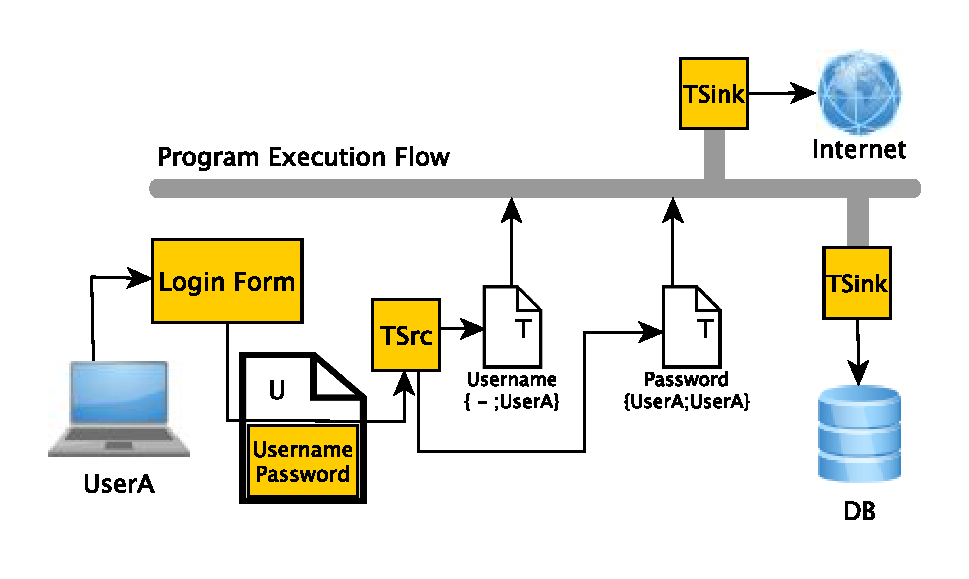
\includegraphics[width=0.7\textwidth]{figs/cifc-model}
\centering
\caption{CIFC operation scheme}
\label{fig:cifc-model}
\end{figure} 

For example, a label defined as \texttt{\{\{Alice;Bob\},Alice\}} would mean that both Alice and Bob are able to access data for read purposes but only Alice can alter this data. Also, the label \texttt{\{ - ,UserA\}} (as represented in Fig. \ref{fig:cifc-model} means that the associated data is public for read purposes but only \texttt{UserA} is able to alter it.
So, CIFC allows data-centric security policies to be defined by a central authority, specifying who can read or alter each data item in the system, allowing user's sensitive data to be protected against unauthorized accesses, therefore assuming the central authority responsible for policies definition is trusted and cannot be compromised.

\subsubsection{Decentralized Information Flow Control}
\label{sec:difc-model}
CIFC model described in Sect. \ref{sec:cifc-model} was primarily designed for simple environments where security policies are held and decided by a central authority, which enforces all the users to trust this system component, assuming that it cannot be compromised. It best suits systems where every operation is performed in the same single domain, thus not requiring data to be sent to untrusted third-parties. For example, a university where multiple departments coexist, being each department responsible for defining rules for data owned by itself. As we show below, this scenario cannot be modeled by CIFC, because there is no notion of data ownership, being a central authority responsible for controlling every access. Decentralized Information Flow Control \cite{difc} is a proposed model that improves CIFC by decentralizing the policy checking and holding from a central authority to the users themselves.

The essential parts of the DIFC model are: \textit{principals}, whose privacy the model is designed to protect; and \textit{labels}, the way in which principals specify their desired privacy constrains. DIFC labels, that take the form of \texttt{\{owner: readers\}} extend classic IFC labels by adding a notion of ownership to each label, which is a principal or group of principals that is able to declassify its own data but not to change policies held by other principals. Principals may delegate all their power in other principals, through acts-for relations specifying the new principals that can act on behalf of the original one.

Since these systems have to deal with information entering and leaving the system from/to remote locations, DIFC also extends these policy checks to the communication channels that support this data exchanges, associating them labels that operate on the input and output of data through these channels, with the purpose of not having any unlabelled data inside the system. When some value is read from an input channel, this value will be initially assigned with the label of the channel. On the other hand, a value can only be written to an output channel if the channel's label is at least as restrictive as the value's label, preventing this way information leaks through unprivileged communication channels.

DIFC base concepts and operation are demonstrated on Fig. \ref{fig:difc-model}, taking as example scenario an university management platform in which their students receive all the exam marks by e-mail. This example has the importance of showing how some common scenarios cannot be modeled by CIFC. The teacher corrects the exams, and when he finishes, he marks the exams as corrected. At this time, the exams are automatically sent to the university secretary that is responsible for sending the e-mails to the students with the corresponding marks. Also, the university has a private statistics bank where all the marks are compiled every year on performance reports that compare the students' success with previous years.

\begin{figure}[t!]
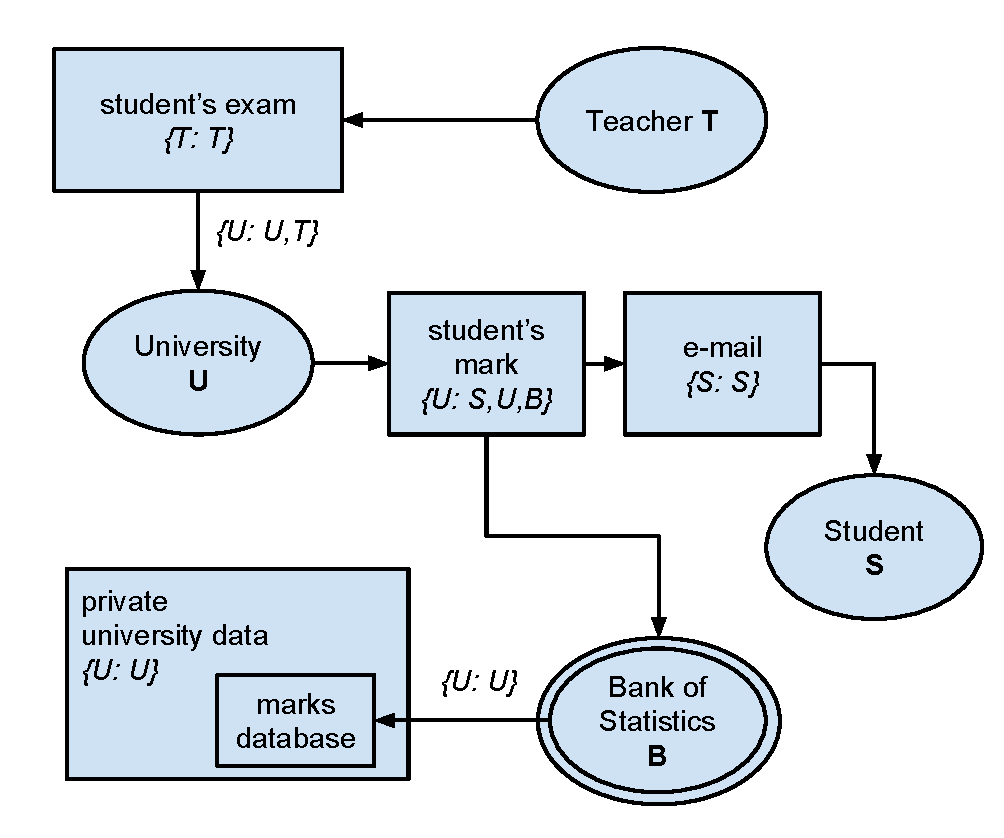
\includegraphics[width=0.7\textwidth]{figs/difc-model}
\centering
\caption{DIFC operation example}
\label{fig:difc-model}
\end{figure}

This is an example of a scenario where DIFC suits better than simple IFC, since the system is composed by multiple parts that not necessarily trust each other, as for example, a student may want to be sure that his marks are not leaked to other students. Also, a teacher may not want the university to be able to access the exam before he finishes the correction.

Modeling these restrictions in a DIFC model, we can find four principals, represent by ovals, which can hold data and need protection for that data: Teachers (\texttt{T}), University (\texttt{U}), that represents the university secretary, Student (\texttt{S}), and the Bank of Statistics (\texttt{B}) responsible for compiling and saving the statistics reports and which benefits from special trust by the university and the students, the reason why it's represented with a double oval.

The teacher corrects the exams, and when he finishes, the label \texttt{\{T: T\}} is assigned to the exam, specifying that the teacher is the owner of the exam and also only him is able to read it. When he finishes the correction, he gives the ownership of the exam to the university, but still keeps his ability to consult the exam. The university then takes the mark from the exam, composes an e-mail that is owned and only readable by the student \texttt{\{S: S\}} who will receive it, being sure that his information was not leaked anywhere else. Apart from that, the university makes the mark available for the bank of statistics to read, so it can be stored in the university database.

The bank of statistics has the authority to act on behalf of the university (\texttt{U}), so it can replace the student mark's policy from \texttt{\{U: U,B,S\}} to the statistics policy \texttt{\{U: U\}}, such that the mark can be saved in the statistics database and only accessible by the university.

In this scenario, there occur declassification in four situations. In first place, when the teacher transfers the exams ownership from himself to the university to process them. Then, the university composes an e-mail to be sent to each student carrying his mark, declassifying the e-mail to be owned and readable by the student only. At the same time, the university declassifies the mark, making it available for the bank of statistics to read, in order to include it in the yearly report. Finally, the bank of statistics endorses the mark's security, transferring the ownership of the mark to the university again, so it can be stored in the private database. In each situation, we are applying the rule that a principal may only modify the policies owned by itself, not present in centralized information flow control, which is the reason why it cannot model this scenario.

\subsubsection{Discussion}
In this section, we discuss which of the presented information flow control models better suits our mobile application target scenario.

Multiple similarities can be spotted between this scenario that suits the DIFC model for privacy protection and the examples of applications that exchange sensitive information about their users and that we approach as targets for the Floodgate. Foremost, the multiple principals that comprise the scenarios can be compared as current applications that rely on multiple third-party services where each one has the responsibility for a part of the whole system functionality and does not necessarily trust the others.

For example, a mobile application that presents location-based suggestions to its users may query a restaurants database for suggestions of where to eat and a monuments database to find the best places to visit. Apart from that, it may still require advertisements from another third-party server, so we consider each one of these parties as a principal in the model. A distrustful relationship is present, since the user may not trust the third-party content providers and these may not trust the application itself.

To address this trust issue, the DIFC system must possess data declassification mechanisms that allow principals to constantly exchanging privileges over information, granting or removing permission to/from other principals to access data. For example, the user location must be protected from third-party leaks, and thus, the user could define that only him and the principals that need to access its location to proffer functionality may access this information. For this reason, we argue that the DIFC model best fits our needs in terms of data tracking, policies specification and enforcement, and so must be seen as good basis for the Floodgate system model.

\subsection{IFC System Design Space}
\label{sec:ifc-system-design-space}

Since the concept of IFC was proposed, multiple systems and techniques emerged, differing between them on key design issues, which, according to Bacon et al. \cite{bacon2014}, can be summarized on the following questions:

\begin{enumerate}
\item When the system operates?%(static, runtime, hybrid);
\item Which granularity the system operates at?% (e.g. domain level, process level, variable level, message level);
\item How the system enforces data isolation?% (hardware-assisted OS, programming language libraries);
\item How the system specifies data policies?
\end{enumerate}

\subsubsection{1. When the IFC System Operates?}
An IFC system may be a static method if its operation occurs at the program compilation time or a runtime method if it operates dynamically when the program is running, accepting data exchanges in and out of the system. Finally, a hybrid method comprises at least two components, extending the method operation at both compilation time and runtime.

\textbf{Static methods} provide a way to verify the correctness of cloud components and all the interactions that happen between them. These mechanisms allow cloud providers to guarantee a trusted base on top of which their clients can deploy applications. Despite they are not effective in enforcing end-to-end privacy protection on runtime, during dynamic arrival of application inputs, these methods are immune to IFC threats like timing or termination channels. As examples of static methods we outline:

\textbf{Static taint analysis}, implemented in Pixy \cite{pixy}, a technique that analyses a target program in order to check that every accepted input is sanitized before it can be considered as safe to be applied in the system operation. It attempts to prevent attacks like SQL injection or Cross-Site Scripting (XSS) \cite{xss}. Also, \textbf{security-Typed Languages}, such as Haskell \cite{haskell}, allow application developers to explicitly define security policies attached to the type of each variable while writing the application code. The compiler enforces to take these confidentiality and integrity policies at program compilation time.

\textbf{Runtime IFC methods} are techniques to achieve data labelling and taint tracking while a program is running. Despite they add a runtime overhead due to the taint tracking mechanisms, these systems are able to detect potential dangerous information flows, in which sensitive information belonging to users might be leaked or malicious data might damage the system itself.

TaintDroid \cite{taintdroid} is an example of a runtime method, which monitors Android applications while running. It detects when applications try to exfiltrate data coming from sensitive information sources (i.e., device location sensor, user phonebook), reporting the responsible application, data type and network destination to the user.

Apart from purely static and purely runtime systems exemplified above, there are special cases known as \textbf{hybrid methods} because of their operation both at compile and runtime.

Jif \cite{jif} must be seen as a hybrid system that divides its functionalities between both compile and runtime. Jif is an example of a security-typed language which extends Java by adding DIFC labels to the data type system. These labels define a set of rules that a program must follow in order to prevent sensitive data leaks. Then the compiler verifies all program statements based on DIFC labels, which include compile-time checks (static component) of whether data with a certain associated label reaches another variable or a communication channel associated with a more permissive label, generating compilation errors in such case. Apart from that, Jif allows ownership and permissions over data to be granted and checked by the system in runtime, which is useful in systems where information flow cannot be verified statically and privileges over information may change over time.

\subsubsection{2. Which Granularity the System Operates at?}

Current IFC systems often divide an application into multiple isolated components that vary on their contribution to the whole application and on the security-level required to interact with them. Generally, data inside an application flows across isolated components, possibly exchanging labels and metadata on each transition, so it is essential to intercept the exchange of data, analyze the intercepted data and update information flow metadata accordingly, if necessary. IFC tracking can be enforced at different granularities and systems must determine a balanced way of providing effective data tracking while minimizing additional verified overhead.

\paragraph{A) Tracking at VM Level:}
Considering an architecture where multiple virtual machines controlled by a hypervisor run different applications, there is the need to control how data flows between virtual machines and also interactions with the hypervisor. Payne et al. \cite{payne} proposed a layered model for security policies, in which every request between VMs running over the same hypervisor is associated with two labels. One label is assigned by a guard component responsible for inspecting the request type and content, and the other one, derived from the first, is assigned by the hypervisor stating whether the request may reach the destination VM. This distribution is done in order to lower complexity by reducing the relations verified at each layer.

\paragraph{B) Tracking at Process Level:}
A fine-grained approach, tracking at process level allows taint tracking to intersect and verify data exchanges between different applications installed on the same device, requiring each one to be encapsulated on its own process. This way, every interaction between different processes is intercepted and analyzed by the data flow tracking system. It is used in Asbestos \cite{asbestos}, Flume \cite{flume}, HiStar \cite{histar}, Nexus \cite{nexus}, Laminar \cite{laminar}, DStar \cite{dstar} and almost all DIFC-driven operating systems, but also suffers from little adoption since it requires a deep change on the application's development environment and it is not capable of tracking suspicious interactions within the same software component as a variable-level approach do.

\paragraph{C) Tracking at Variable Level:}
Providing data flow tracking at variable level, allows every variable defined in the context of an application to be monitored, preventing unsafe uses. Jif \cite{jif} language attaches to each variable a pair of labels composed by a confidentiality label and an integrity label. These labels are checked on each interaction between components and data holding them may be endorsed or declassified, based on the privacy needs at each moment, defining the possible flows an application can securely allow. Even in the presence of incorrect or malicious software implementations, if labelling is correctly defined, a user trying to read another's confidential data will be presented with an exception indicating the invalid request made.

\paragraph{D) Tracking at Multiple Levels:}
IFC systems designed to operate exclusively at mobile side usually combine multiple of these approaches to achieve an efficient data tracking. Uppermost, the OS running on mobile devices is slightly different from general Linux distributions widely used to power servers on which applications base their functionality. Also, contrary to what happens on Linux, applications running on mobile operating systems must be written in one specific language that provide interfaces to communicate with the device itself, in order to gather information. On Android systems, applications are written in a modified version of Java language, and thus, IFC systems designed to operate over Android \cite{taintdroid,pebbles,mockdroid} know a priori which language libraries and variables to track. Apart from variable/library-level tracking, Android-supported IFC systems also perform tracking at interprocess message-level, since each application runs on its own Dalvik VM encapsulated in a process, which results in a way of controlling how taints are propagated between applications. Finally, as every Android device runs its own filesystem where application data is often persistently stored in files, these systems also perform tracking at file-level, keeping security labels hooked to the corresponding files. This file-level tracking is crucial for the system effectiveness because files often contain much more information than variables. In conclusion, mobile IFC systems maintain users privacy by acting as all-around privacy protection mechanisms for mobile devices.

\subsubsection{3. How the System Enforces Data Isolation?}
Data isolation is an essential mechanism to complement data flow tracking and analysis, since it prevents data from being exported through unexpected channels or flowing into undesired system components without previous security monitoring and sanitization. For example, a secure container encapsulates the execution of an application so that data is securely accessed and input/output is checked for security purposes. The goal of data isolation mechanisms is to only allow data exchange when the application requirements strictly need it. To achieve data isolation, the following approaches have been studied:

\paragraph{A) Isolation Through Virtualization:}
On a virtualized environment, isolation is performed at the virtual machine level and enforced by both the hardware and the hypervisor. The CLAMP system \cite{clamp} provides a virtualized environment to applications built under the popular Linux, Apache, MySQL, PHP/Perl (LAMP) stack, allowing developers to continue using the operating systems, platforms and languages they are used to. CLAMP uses the Xen hypervisor to isolate each user's data on a virtual dedicated web server instance, only accessible through authentication on a developed module. The database queries performed by the user are restricted a trusted Query Restrictor that guarantees that only data owned by the user assigned to the querying web server can be accessed.

\paragraph{B) Isolation Through Programming Languages and Libraries:}
In opposition to isolation achieved at the VM-level, recent implementations of IFC systems allow developers to explore the taint-tracking facilities present in languages like Ruby and Perl to enforce data isolation at the best possible, since it cannot be strictly enforced. These approaches have the advantages of isolating data just by interacting with already defined language libraries, discarding the need to adapt the runtime environment to accommodate desired isolation features. SAFE WEB \cite{safeweb} uses Ruby dynamic features, like safe levels. Safe levels can restrict the execution mode of Ruby code on different kinds of isolated environments, through a \$SAFE variable that has 4 isolation levels (level 4 means no I/O operations). Relying on this, SAFE WEB achieves label propagation and data flow enforcement, but it is primarily suitable for detection and protection against unintentional software bugs than to deal with explicitly malicious application code from unreliable third-party providers.

\paragraph{C) Isolation at \textit{Middleware} Level:}
Designed for multi-tier web applications in which data has to flow between multiple sub-systems, called domains, event-based IFC systems define messages between these domains as events. SAFE WEB is an example of an event-based IFC system which apply an event-level or message-level granularity in data flow isolation. In these type of systems, events between domains are often placed in an event broker by the sender domain, and the event broker handles the task of delivering events only to interested domains that are allowed to read the event information, being this event broker the only way how domains are able to exchange messages.

\subsubsection{4. How the System Specifies Data Security Policies?}
A basis option to take in the designing of an IFC system is to specify how security policies are unambiguously defined. Currently used examples are policy-definition languages or \textit{ad-hoc} definitions, specific to each system. 

\paragraph{A) Policy-Definition Languages:}

Policy-definition languages allow the specification of ``can-flow-to'' relations between DIFC labels, applicable in the context of every application, just by having the knowledge of principals present in the application. JFlow \cite{jflow} is a policy-definition extension for Java language that allows the programmer to define allowed relations between labels under a usable programming model, making it simple to use.

\paragraph{B) \textit{Ad-hoc} Policy Definition:}
In contrary to what happens with the usage of languages to specify security policies, an ad-hoc policy definition means that security policies are specified by the developer itself, that is responsible for writing policy checking code. RESIN \cite{resin}, is an example of an \textit{ad-hoc} policy definition system, allowing programmers to create \textit{policy objects}, which specify assertions associated with application data to be checked when data crosses certain data flow boundaries (i.e., in an attempt to send data over the network).

Throughout the time, there emerged some real systems that implement the IFC models described above. We now present the most representative cases, based on Floodgate's context which implicates three different types: Systems which operate on the mobile-side only, others that do it exclusively on the server-side and also the distributed approaches, which implicate data communication between two entities. 

\section{Mobile-side IFC Systems}
\label{sec:mobile-ifc-systems}

For the mobile-side, we chose three systems which take different approaches: TaintDroid, Aurasium and FlowDroid.

\textbf{TaintDroid} is an extension to the Android mobile operating system capable of tracking the flow of sensitive data across downloaded third-party applications. TaintDroid aims at informing mobile devices' users of how these applications make use of permissions granted on installation.

TaintDroid regards two main goals: The detection of when sensitive data, like user's location or information about the device, leaves the system through third-party applications that might send it to remote locations on the network. The other one is to facilitate application security analysis by device users or external security auditors. With TaintDroid, a user can easily verify whether an application performs active intents to leak its private data.

An approach through static source-code analysis is infeasible, because most applications are closed source and often are realtime changeable configurations that dictate application's behavior. So, TaintDroid uses \textit{dynamic taint analysis} to monitor privacy sensitive data on mobile devices. TaintDroid knows \textit{a priori} the sets of taint sources and sinks present in the device.

Firstly, information coming from a \textit{taint source} (source of sensitive information, like the GPS sensor) is identified and a \textit{taint marking} indicating the information type (location-sensitive, contact-sensitive) is assigned. Then, dynamic taint analysis perform an instruction-level tracking on how labelled data interacts with other data over the application information flow in a way that might cause the leakage of the original data. Finally, all the impacted data is identified when an intent of leaving the system through a \textit{taint sink} (normally the network interface) is detected.

Taking advantage of virtual-machine-based smartphones architectural characteristics, TaintDroid provides an efficient, system-wide taint tracking mechanism, illustrated in Fig. \ref{fig:taintdroid-arch}. In first place, the VM interpreter is instrumented to provide \textit{variable-level} tracking within the application code. Then, \textit{message-level} tracking between applications is used, since applications are allowed to share data between themselves through Binder, i.e., the Android component responsible for IPC. Third, for trusted system-native libraries, TaintDroid uses \textit{method-level} tracking, running code without instrumentation and applying the taint propagation on the method return. Finally, \textit{file-level} tracking is used to ensure that information stored persistently also keeps the assigned taint markings.

\begin{figure}[t!]
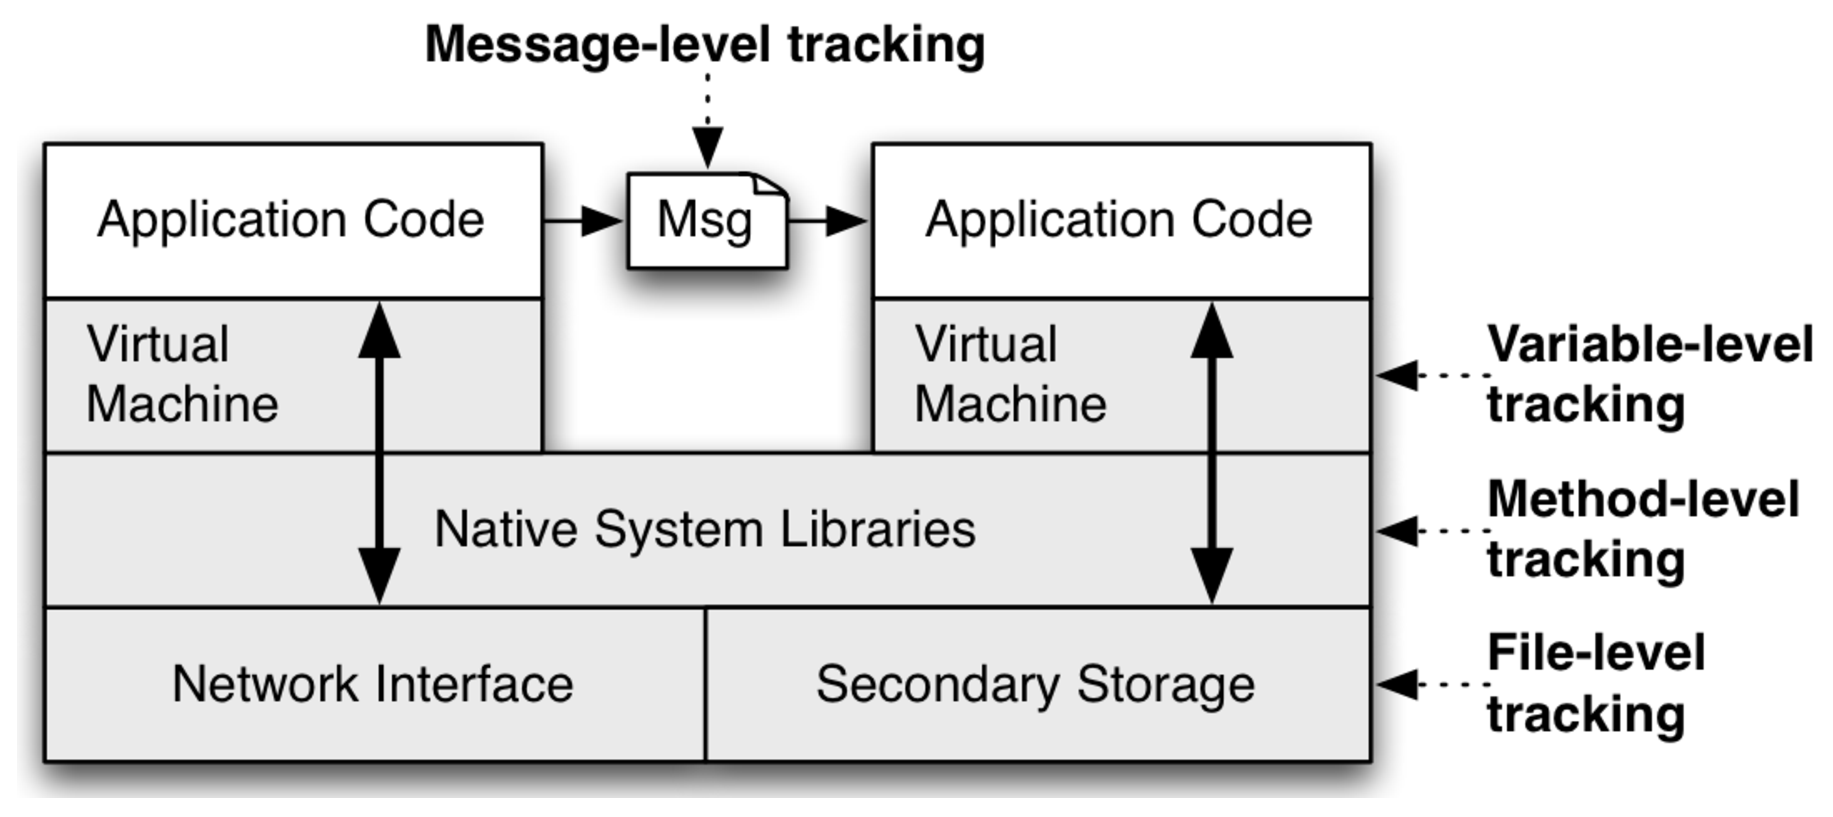
\includegraphics[width=0.7\textwidth]{figs/taintdroid-arch}
\centering
\caption{TaintDroid tracking system overview}
\label{fig:taintdroid-arch}
\end{figure}

To ensure that applications are not capable of maintain sensitive untracked data flowing in the system, TaintDroid assumes that the TCB is comprised only by the virtual machine (not the code) executed in user-space where applications operate in and the operating system, or more specifically any native system libraries loaded by the untrusted interpreted application. This way, TaintDroid modified the original Android platform to only allow applications to escape the virtual machine through native libraries that are, therefore, trusted.

Figure \ref{fig:taintdroid-arch-2} gives a detailed view over the TaintDroid architecture. After information is tainted (1) on a trusted application that carries enough context to perform the taint operation (the location-provider, for example), the taint interface invokes a native method (2) that interacts with the Dalvik VM interpreter, storing some specified taint markings in the \textbf{virtual taint map}. The Dalvik VM is then responsible for propagating taint tags (3) according to data flow rules, while the application uses the tainted data in its operations. Multiple interpreters may be propagating taint information, as many applications may be running at the same time. By the time that the trusted application uses the tainted information in an IPC call, the Binder IPC Library (4) ensures that the data archive containing all data to be transferred has a \textbf{taint tag} reflecting all the taint markings of all associated data. If true, the Binder Kernel Module (5) performs the dispatch of the data, which will be received by the IPC library on the untrusted application side. This library then removes the taint tag from the data archive and assigns it to every data contained in it. The Dalvik VM interpreter then propagates the taint markings (7) on the untrusted application side, identically to what happens on the trusted side and anytime the untrusted application invokes a library (8) known as part of the taint sinks set (e.g. network interface), this library reads the taint tag from data referred in the invocation (9) and reports the event, describing the exported data, its destination and the associated taint tag.

\begin{figure}[t!]
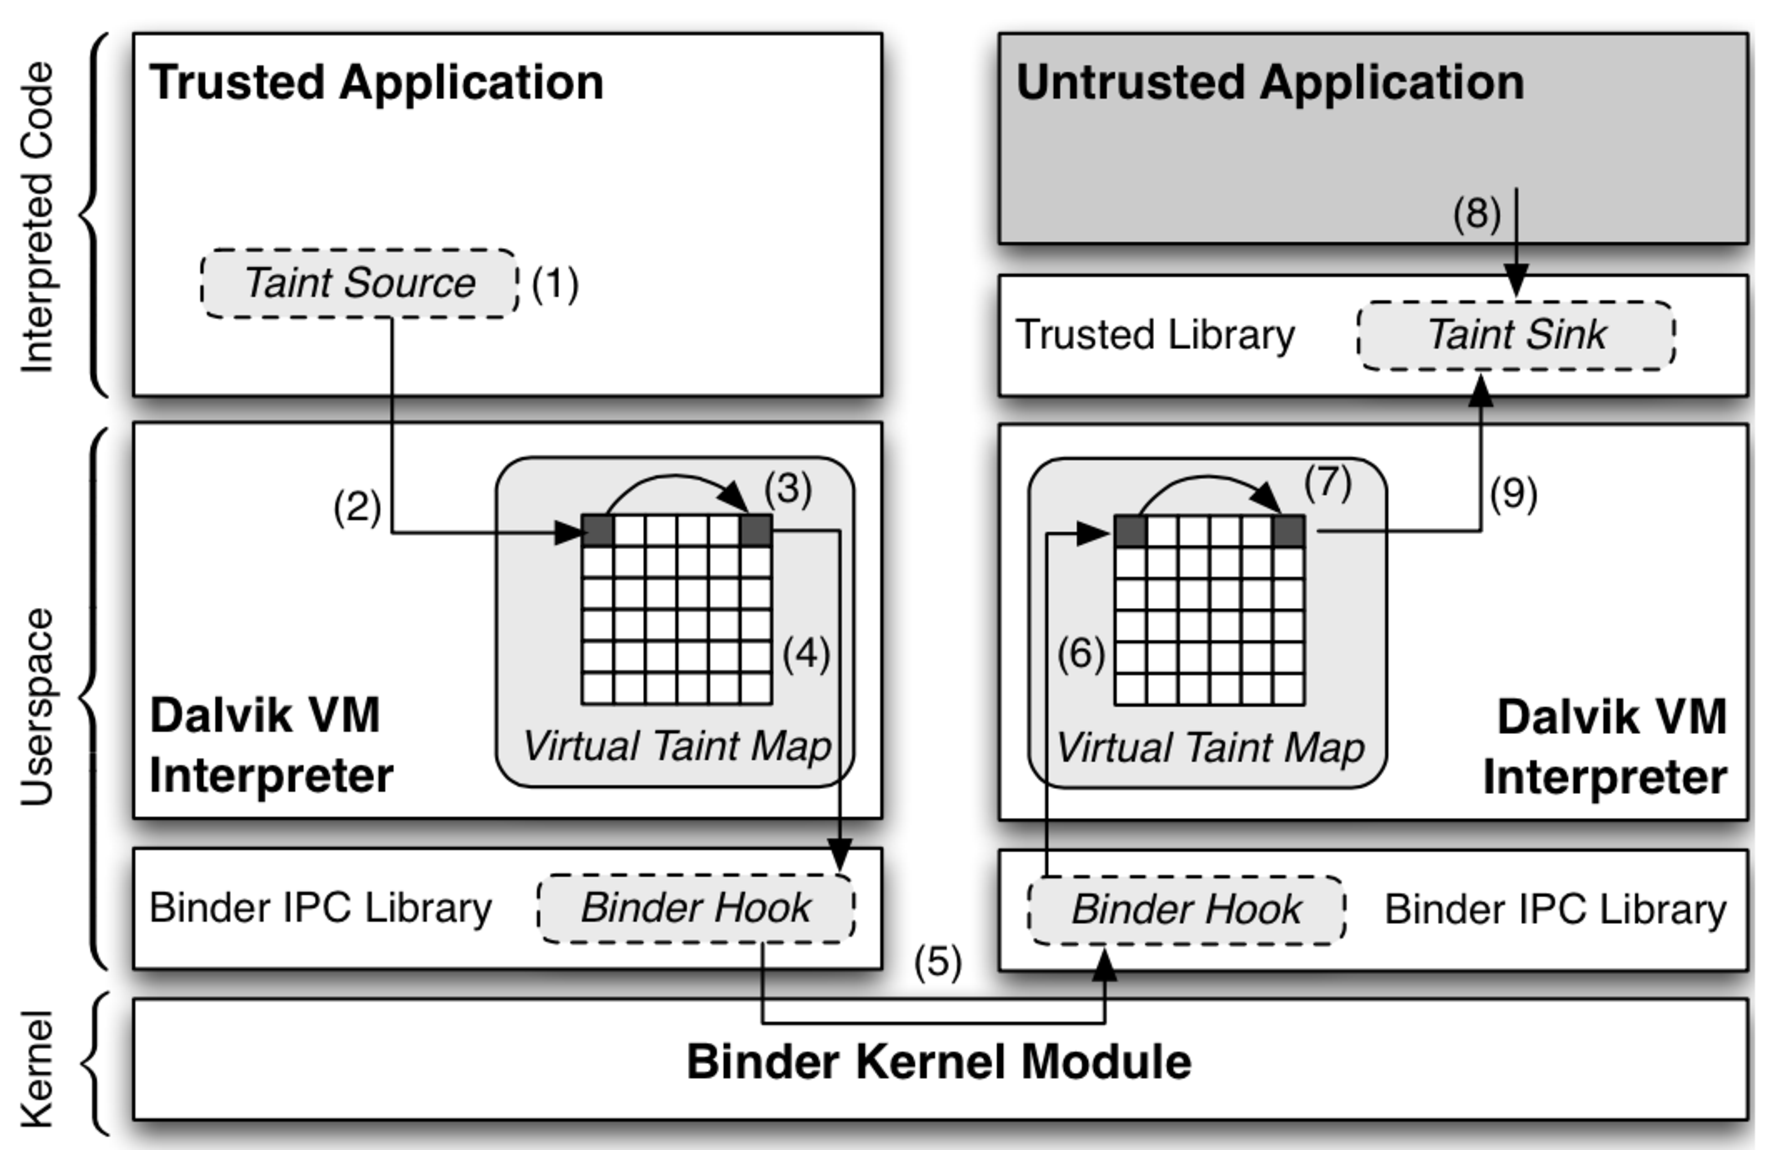
\includegraphics[width=0.7\textwidth]{figs/taintdroid-arch-2}
\centering
\caption{TaintDroid architecture}
\label{fig:taintdroid-arch-2}
\end{figure}

TaintDroid stores taint tags in memory positions adjacent to variables, like class fields or arrays, providing spatial locality that might influence the system performance positively. Also, only one taint tag is stored per array, which minimizes storage overhead but may lead to false positives, since if an array contains only one tainted data object in a given position, the whole array must be considered as tainted.

Against the stock Android platform, TaintDroid revealed a 3\% performance overhead in starting an application, 5.5\% and 18\% increased time for address book create and read operations, respectively, 10\% overhead in making a phone call and 29\% overhead on taking a picture with the device camera. Also, an IPC benchmark revealed that for a set of 10.000 messages exchanged between client and server applications performing binder transactions, TaintDroid is 27\% slower and uses 3.5\% more memory.

TaintDroid presents an efficient approach to track information flows on Android systems. The dynamic taint analysis method offers effectiveness on tracking how information coming from taint sources are used throughout the application, relieving the need to trust the application itself. Also, the spatial locality provided by the taint tag storage method minimizes the added overhead. Although, TaintDroid is not effective in preventing the exfiltration of sensitive data, since it only builds a report of situations when it occurs, instead of blocking network access in such cases, which is included in Floodgate's goals.

The second mobile IFC system we present is \textbf{Aurasium}, which may be described as an application-hardening service. It is intended to be used in order to turn untrusted Android applications, downloaded from third-party providers, into secure applications enforcing policies regarding the user's sensitive data privacy. In order to achieve that, the system relies on a repackaging process of the application package, and the output is a hardened version of the same inputted application to be directly installed on a device.

In practice, Aurasium takes advantage of Android's application design of mixed Java and native code execution to introduce \textit{libc} interposition code to the target application, wrapping around the Dalvik VM under which the application's Java code runs. This way, Aurasium is able to intercept almost all interactions between the application and the operating system, since most of them trigger the execution of native methods, which is often transparent to developers, due to the available APIs. Also, code modification is used in order to place the interposition code whenever the application starts. Figure \ref{fig:aurasium-arch} illustrates the space where the system acts in the Android OS context.

\begin{figure}[t!]
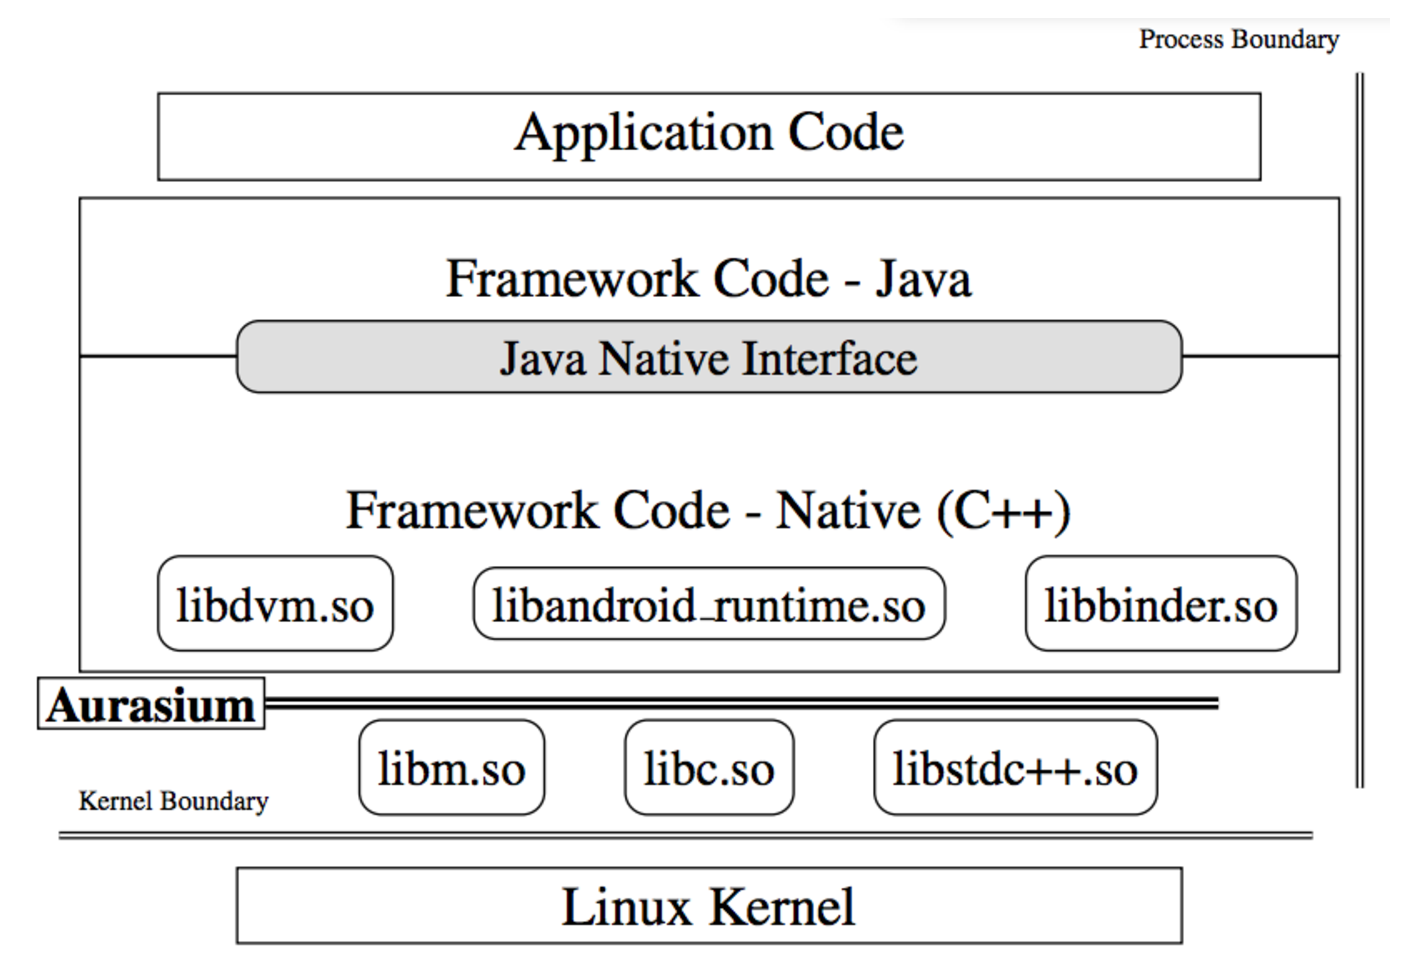
\includegraphics[width=0.7\textwidth]{figs/aurasium-arch}
\centering
\caption{Aurasium action context}
\label{fig:aurasium-arch}
\end{figure}

In Aurasium, the security policies are enforced, for example, whenever an application tries to communicate with a remote endpoint through the network. In such case, Aurasium first checks it against an well-known IP blacklist, frequently updated. Also, whenever an application
tries to access the device's IMEI, as illustrated in Fig.  \ref{fig:aurasium-policy}, a policy check is performed to allow or disallow the access. These policies are included in the self-contained final application package and may save its state and check it in future occasions. Aurasium's interposition code shows a dialog to the user, asking whether permission to perform an action which might violate the security policies should be granted.

\begin{figure}[t!]
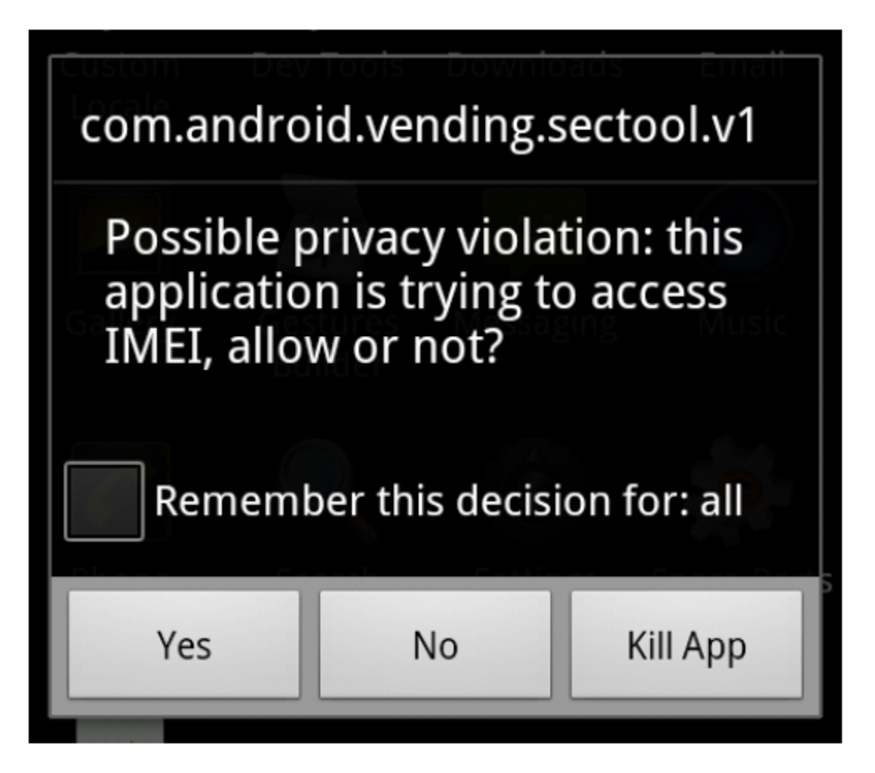
\includegraphics[width=0.5\textwidth]{figs/aurasium-policy}
\centering
\caption{Aurasium policy example}
\label{fig:aurasium-policy}
\end{figure}

In order to produce the hardened version of an application to be run in the same devices as its non-secure version, Aurasium first needs to decompile the application's compiled bytecode, which is stored in a single file called \texttt{classes.dex} inside the application's \texttt{APK} package. After that, the code is inserted in normal Java classes and the application entry point is set to the Aurasium \texttt{Application} class, which guarantees that Aurasium becomes the application's entry point and its sandbox is established before the application can perform any other action. Figure \ref{fig:aurasium-repackaging} shows the components of a common \texttt{APK} package and the Aurasium components introduced during the repackaging process.

\begin{figure}[t!]
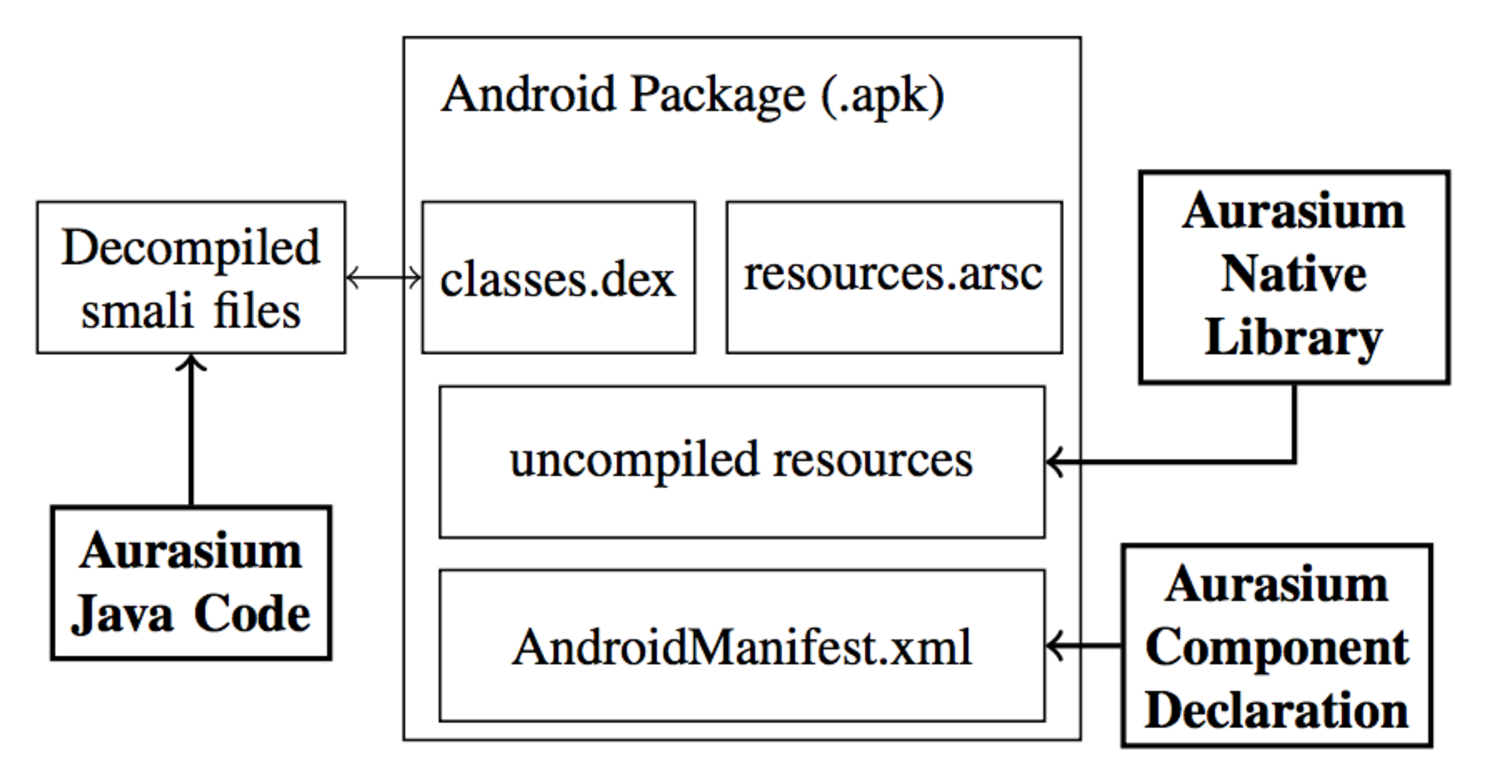
\includegraphics[width=0.7\textwidth]{figs/aurasium-repackaging}
\centering
\caption{Aurasium repackaging process}
\label{fig:aurasium-repackaging}
\end{figure}

After the repackaging process, the final step is resigning the application package, since every Android application is required to have a valid signature, which proves its authorship. To maintain this, Aurasium keeps the application's old signature (before the repackaging), and then verifies its validity. If it is valid, then the application is re-signed with its old signature. If don't, then Aurasium will use a randomly-created signature, which will not keep the application's authorship information.

To complement, Aurasium features a helper application, named Aurasium Security Manager, which users may install in order to centrally manage permissions granted/revoked to their Aurasium-packaged applications. For instance, if a user permanently decided to not let a given application access his phone number, with this helper application they may change it in the future.

In terms of performance, Aurasium shows worse results when applications perform a large number of requests to the underlying Android APIs, with an overhead of 14\% to 35\% on three use-cases, specifically developed to perform a lot of API invocations. In terms of size of the hardened application package, Aurasium showed a constant increasing of about 52 Kb, which the authors considered a minor overhead.

In conclusion, Aurasium tries to achieve practical security enforcement and contributes with its novel repackaging process and a set of policies regarding sensitive mobile information. This system shares with Floodgate the goal of not requiring changes on the mobile operating system in change for protection, avoiding problems regarding the system's adoption and cross-version compatibility.

The third mobile IFC system we present is \textbf{FlowDroid} \cite{flowdroid}.

\section{Server-side IFC Systems}
\label{sec:server-ifc-systems}

\section{Distributed Approaches}
\label{sec:distributed-ifc-systems}

\section{Discussion}
\label{sec:related-work-discussion}
 
 

%%%%%%%%%%%%%%%%%%%%%%%%%%%%%%%%%%%%%%%%%%%%%%%%%%%%%%%%%%%%%%%%%%%%%%%%%%%%%%%%%%%%%%%%%%%
%                               My System 24pp
%%%%%%%%%%%%%%%%%%%%%%%%%%%%%%%%%%%%%%%%%%%%%%%%%%%%%%%%%%%%%%%%%%%%%%%%%%%%%%%%%%%%%%%%%%%
\chapter{Architecture}
\label{sec:Architecture}
 
%%%%%%%%%%%%%%%%%%%%%
 
\section*{Summary}

In this chapter we will present the details we propose regarding Floodgate's architecture. In first place, on Sect. \ref{sec:floodgate-overview}, we will present a brief overview of our system. Then, in Sect. \ref{sec:building-blocks}, we will present and justify the building blocks in which our mobile-server architecture is based, talking about the IFC models implemented on each end. After that, we will present the programming and deployment model which developers must follow in order to produce Floodgate-ready applications, on Sect. \ref{sec:programming-model}. Then, we will provide a detailed explanation of how we achieve the end-to-end taint tracking and how we deal with taint persistence on the server-side, on Sect. \ref{sec:end-to-end-taint-tracking} and \ref{sec:server-side-taint-persistence}, respectively.

In the next chapter we present the implementation details for the proposed architecture.

\section{Floodgate Overview}
\label{sec:floodgate-overview}

We propose Floodgate, a system that will rely on a mobile-server architecture to ensure the end-to-end enforcement of specified security policies (SP) across the whole system, as represented on Fig. \ref{fig:floodgate-arch}. Compared to the existing systems, Floodgate will work at \textit{middleware-level}, enforcing security policies in an end-to-end way between mobile-side applications and server-side \textit{backend} supporting those applications. In Floodgate, security policies are specified by the service provider and accepted by the user upon the installation of a mobile application supported by our system (1). On one side, the mobile device running the Android operating system performs an application-level tracking of sensitive data across third-party applications, adding policy checks that prevent the undesired exportation of private data, accordingly with specified security policies. By application-level tracking we mean that, in Floodgate, we follow a more coarse-grained tainting approach, applying taints to the whole application instead of data variables present in the application's data flow. When the application is marked as tainted and data is sent to remote \textit{endpoints} (2) through the taint sinks (e.g. network interfaces), this data has to keep the application's taint marks and security policies assigned, in order to achieve the enforcement of those policies on the application server-side. The server-side operates inside a secure container that is responsible for the policies' enforcement and which provides data declassification mechanisms for secure content sharing between applications running in the same container (3) and support for third-party applications interaction (4).

\begin{figure}[t!]
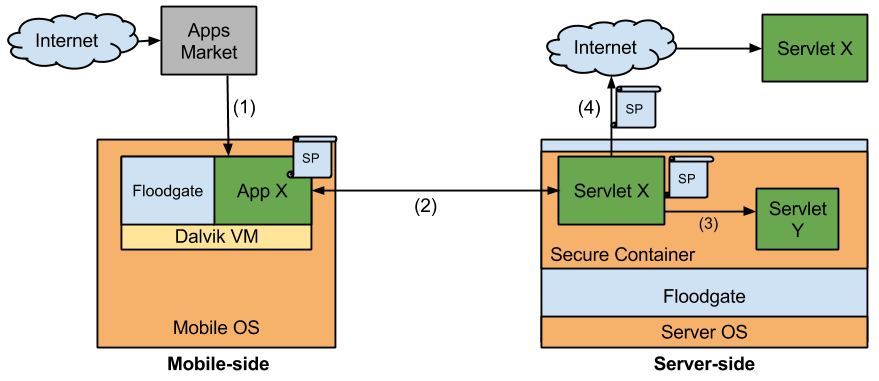
\includegraphics[width=\textwidth]{figs/floodgate-arch}
\centering
\caption{Floodgate proposed architecture}
\label{fig:floodgate-arch}
\end{figure}

\section{Building Blocks}
\label{sec:building-blocks}

As stated in Sect. \ref{sec:floodgate-overview}, Floodgate relies on a mobile-server architecture with components operating on each side. Due to that, we can spot two distinct building blocks, which we now detail.

\subsection{Mobile-side Blocks}
\label{sec:mobile-side-blocks}

On the \textbf{mobile-side}, Floodgate extends common mobile applications with two components, in order to achieve the application-level taint tracking: A text file \textbf{permissions manifest} that is produced by the developer and included in the application's resources; and a library archive, to be specified as a target application's dependency. Both components and the way they interact with the mobile application are represented in Fig. \ref{fig:floodgate-mobile-blocks}.

\begin{figure}[t!]
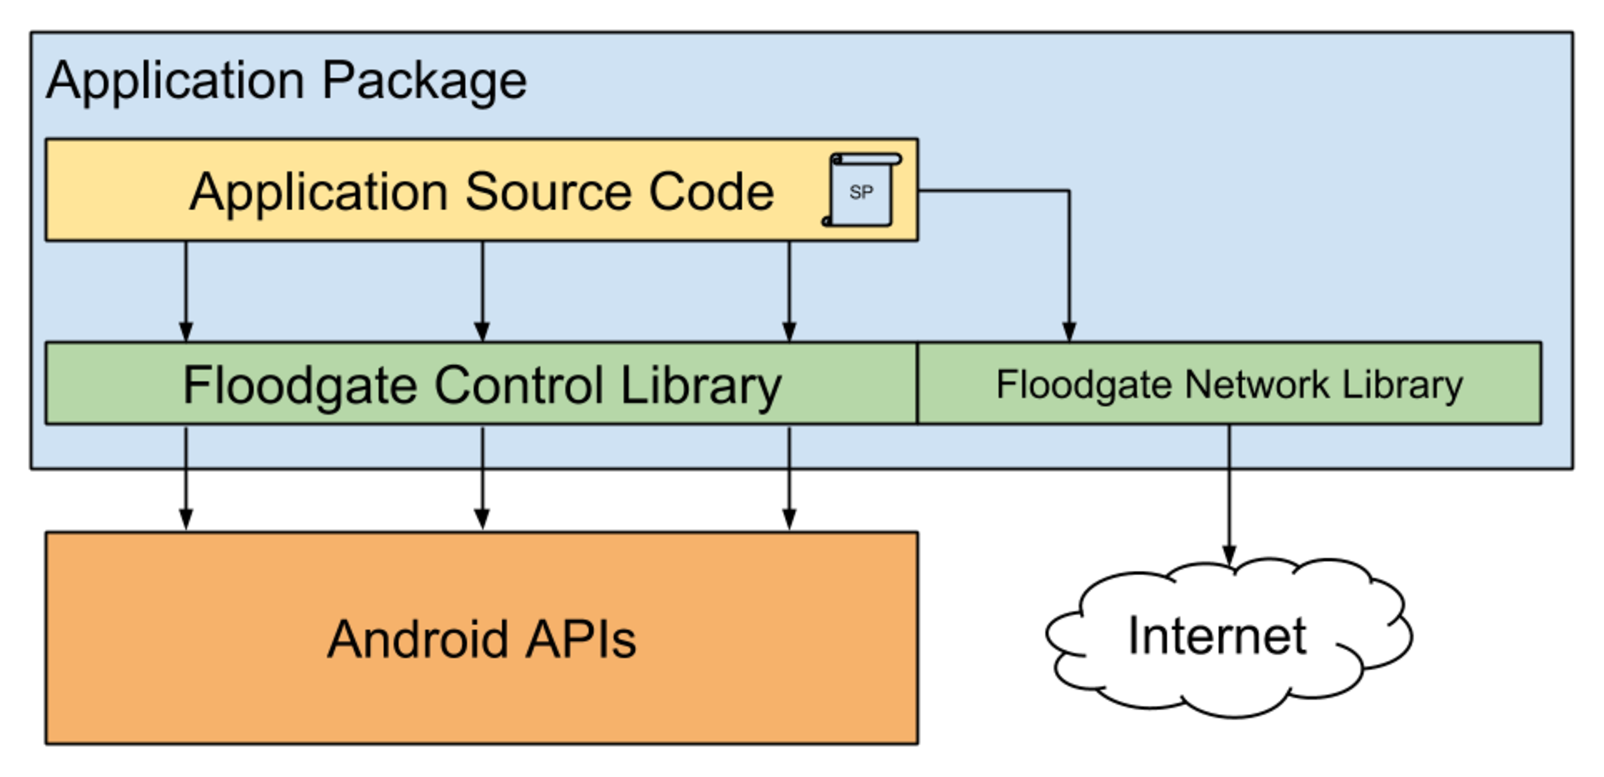
\includegraphics[width=0.6\textwidth]{figs/floodgate-mobile-blocks}
\centering
\caption{Floodgate mobile component design}
\label{fig:floodgate-mobile-blocks}
\end{figure}

The permissions manifest (SP in Figs. \ref{fig:floodgate-arch} and \ref{fig:floodgate-mobile-blocks}) is a data structure which specifies multiple sensitive mobile resources (the device's IMEI, GPS/GSM location, phone number, etc.) along with a key defining the privacy of each resource (public/private). Also, it specifies a list of trusted network \textit{endpoints} with whom the application is allowed to share private resources with. In Floodgate, a public resource is allowed to be sent through the network to any \textit{endpoint}, while a private resource can only be sent to \textit{endpoints} listed as trusted.

The Floodgate's library, by its turn, is comprised by two modules: The control library, which contains the behavior of controlling the access to the resources specified in the permissions manifest and their propagation, and network library, which enables communication over the network. Since Floodgate actually performs an application-level taint tracking on the mobile-side, this library initializes a data structure containing the application taint. This taint is updated when accesses to sensitive resources, specified in the permissions manifest, are detected. In order to detect when the sensitive resources are accessed, the library relies on aspect-oriented programming (AOP) concepts.

AOP relies on partitioning program logic into multiple ``concerns'' (cohesive areas of functionality). With AOP, it's possible to define source code blocks (``cross-cutting concerns'') to be executed before/after/instead another piece of code without explicitly changing it. This way, the ``cross-cutting concerns'' can be implemented once and injected wherever it is needed. The combination of the particular point in a program that might be the target of code injection and the code to be injected is called an \textit{aspect}. Then, the process of injecting code is called \textit{weaving}.

Our library features multiple concerns to be injected when the execution of methods that access a sensitive resource is detected. On such situations, the application taint is updated, always reflecting the resources accessed by the application's source code.

Apart from that, our mobile library also provides methods to communicate with remote \textit{endpoints} over the network.
\todo{Write the network methods available? (in an abstract way, like post(String, Endpoint), get(Endpoint),...)}
These methods ensure that the application taint is always sent along with data, in a transparent way for the developers. In order to enforce this taint propagation through the network, the library features some ``concerns'' regarding the access to other network libraries instead of ours, blocking its execution.

\subsection{Server-side Blocks}
\label{sec:server-side-blocks}

On the \textbf{server-side}, Floodgate provides a secure container where to deploy the \textit{backend} of mobile applications. As referred in Sect. \ref{sec:mobile-side-blocks}, the Floodgate network library deals with the propagation of application taints to the server-side. 

In order to continue the enforcement of such security policies on the server-side, we apply concepts of static analysis, instrumentation and dynamic taint tracking. Every \textit{servlet} running on the Floodgate's secure container has to pass through an \textit{a priori} process of static analysis, graphically presented on Fig. \ref{fig:floodgate-server-blocks}. This process consists in identifying the points in the application where tainted data enters the system, named taint sources (e.g. interfaces to receive network requests coming from the respective mobile application), where it is passed (e.g. variables assignment, methods return) and where it may leave the system (e.g. output network interfaces, database connectors), which we refer to as taint sinks. After the analysis process, Floodgate instruments the application, applying code injection in order to propagate taints wherever the static analysis process dictates to. Finally, we apply dynamic taint tracking in order to keep track of when tainted data are set to leave the system, acting accordingly. Also, Floodgate features a taint persistence module, ensuring that taints entering the \textit{backend} are persistently stored along with data they refer to, avoiding taint loss due to in-memory storage only.

\begin{figure}[t!]
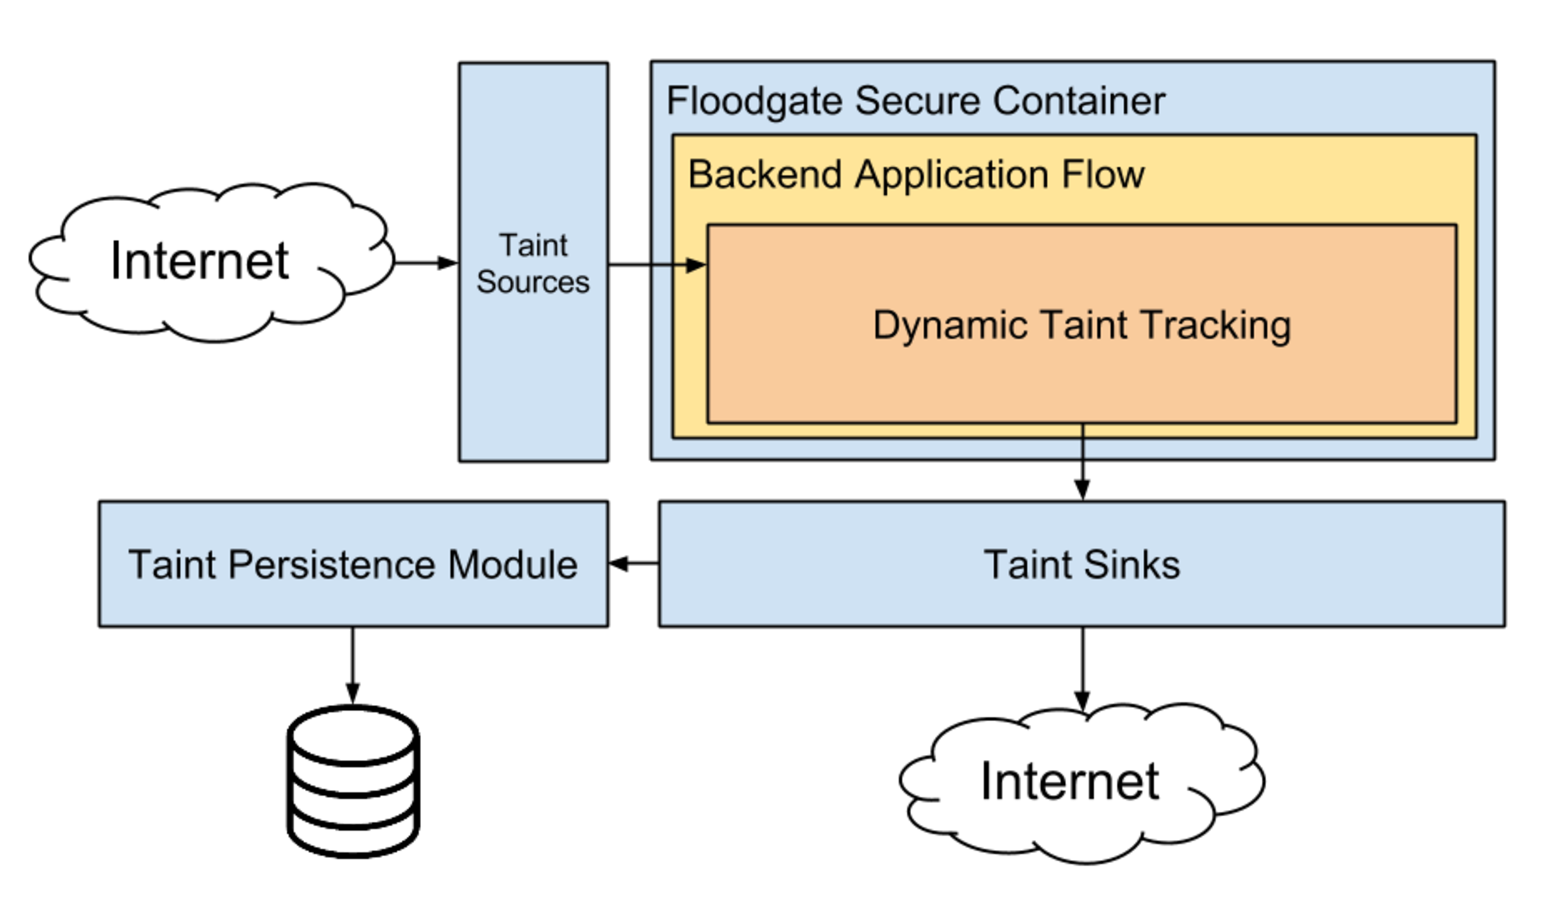
\includegraphics[width=0.6\textwidth]{figs/floodgate-server-blocks}
\centering
\caption{Floodgate server component design}
\label{fig:floodgate-server-blocks}
\end{figure}

\todo{Review the above paragraph. And also, anything more to add? Seems a bit short. The figure also doesn't convince me.}

\section{Programming Model}
\label{sec:programming-model}

Floodgate offers a programming and deployment model specifically targeted to \textit{backend}-supported mobile applications. 

On the \textbf{mobile-side}, the programming model doesn't suffer any major modifications, since developers only need to add the Floodgate mobile library as a dependency for the mobile application and the permissions manifest as an application's resource. After that, developers don't need to worry about anything else regarding data protection and just have to follow normal development process. The only reservation is that developers must use the network methods offered by Floodgate's mobile library to communicate with remote \textit{endpoints}, since they are a key part on the end-to-end taint tracking process. Also, the deployment process for a Floodgate mobile application doesn't suffer any modifications when comparing to the current model.

On the \textbf{server-side}, Floodgate's programming model is essentially based on the definition of a REST API to be deployed on the secure container. This API must offers methods representing CRUD operations to be consumed by the mobile application, which performs HTTP requests (GET, POST, PUT, DELETE) and receives the corresponding responses, with data to be presented at the mobile \textit{endpoint}. Floodgate's \textit{backend} offers an interface to easily define the available API, and the behavior to produce when each API method is called from the mobile \textit{endpoint}. Also, Floodgate offers methods for easily persist inputted data, according to a previously defined database model. Apart from the API-definition interface, the \textit{backend} provides configuration files where developers must define the application data model (e.g. the entities it will handle), the database model and also configuration parameters regarding the \textit{servlet} itself (e.g. the database credentials, ports to be deployed to, security certificates, etc.).

\section{End-to-end Taint Tracking}
\label{sec:end-to-end-taint-tracking}

In this section, we will detail the end-to-end taint tracking process in Floodgate's applications, from the time when the sensitive data is accessed at the mobile device, to when it arrives at the application's \textit{backend}, and on subsequent accesses from there. The process is illustrated on Fig.

When the source code of a Floodgate mobile application tries to access a sensitive data source (e.g. calling the API native method to retrieve the device's phone number), Floodgate's mobile library, and concretely, its \textit{aspects}, will intercept this method's execution. On this interception, Floodgate will verify which of the sensitive methods is executing and then map this method to its corresponding permission manifest resource. This way, Floodgate will be able to check the privacy of the accessed data, relying on the permissions manifest. If the accessed resource is marked as private for the application in question, then Floodgate will update the application's global taint accordingly, initializing it if necessary. In the end, the application taint will contain the information of all the private resources accessed by the application.

When a network method present in the library is called, this method's execution is also intercepted by Floodgate's \textit{aspects}. During this interception, Floodgate firstly verifies the application's taint. If it is not empty, meaning that a sensitive resource was accessed, our system will then verify the destination endpoint for the produced request. This verification includes checking the endpoint's address against the trusted endpoints list present in the application's permissions manifest. If the destination endpoint is not part of this list, then the request will be blocked. Otherwise, if the application is not tainted, the request will proceed with no further checks or restrictions. Summarizing this, if a Floodgate application accesses sensitive data, it will subsequently only be allowed to communicate with trusted endpoints. Otherwise, there are no communication restrictions.

After that, and if the permission to proceed is granted to the request, the mobile library will include the application taint as part of the request, in the form of a header with the name \textit{``privacy''}. This is the way how our system guarantees that the taint tracking is actually performed in an end-to-end fashion. After the HTTP request is composed and the privacy header is appended, then the request will be finally sent.

On the server-side, Floodgate will receive the incoming request, taint data if needed, and enforce the taint tracking during the application data flow. To achieve this, our system comprises an incoming filter for HTTP requests, which examines each request's headers in search for the \textit{``privacy''} one. If the \textit{privacy} header is not empty, meaning that the request contains potentially sensitive data, Floodgate will use its server-side tainting API to assign the \textit{privacy} header taint to the request body.

Following this, the request will trigger a REST API method on the server, using the now tainted request body in the method's behavior. Since Floodgate's server side features dynamic taint tracking, whenever tainted data interacts with non-tainted server data, Floodgate itself takes care of propagating the taints, in order to guarantee the enforcement of the privacy policy on the server-side.

Also, Floodgate features outcoming filters for HTTP requests, which work the same way as the incoming filters but in the opposite direction. So, whenever the \textit{backend} performs an HTTP request, either to respond to the mobile application request or to communicate with other \textit{servlets} (in the same container or third-party ones), the filters also take care of checking taints assigned to data. It is the programmers who must define the security policies regarding situations when applications try to export tainted data, based on multiple available factors such as the data taint or the destination endpoint.

\section{Server-side Taint Persistence}
\label{sec:server-side-taint-persistence}

Apart from taint tracking and enforcement, Floodgate also features taint persistence on the server-side. We achieve this by extending the database model referred in Sect. \ref{sec:programming-model}, in which we include a table for persistent taints. Also, we extend the programming model in a way such that when programmers persist some data, accordingly to the database model, Floodgate automatically persists its taint. Also, when developers query the database model, the returned data is automatically assigned with the corresponding taints, if existing. This allows security policies enforcement even when data is not accessed during long periods of time, and thus not kept in memory.
%%%%%%%%%%%%%%%%%%%%%%%%%%%%%%%%%%%%%%%%%%%%%%%%%%%%%%%%%%%%%%%%%%%%%%%%%%%%%%%%%%%%%%%%%%%
%                               My System 24pp
%%%%%%%%%%%%%%%%%%%%%%%%%%%%%%%%%%%%%%%%%%%%%%%%%%%%%%%%%%%%%%%%%%%%%%%%%%%%%%%%%%%%%%%%%%%
\chapter{Implementation}
\label{sec:Implementation}
 
%%%%%%%%%%%%%%%%%%%%%
 
\section*{Summary}

In this chapter we will present the implementation details and used tools in order to materialize the architecture described in Sect. \ref{sec:Architecture}. On Sect. \ref{sec:mobile-components} we will focus on the implementation of Floodgate's mobile component and leave the server component for Sect. \ref{sec:server-components}.

In the next chapter we present the experimental evaluation of our system.

\section{Mobile-side Components}
\label{sec:mobile-components}

As we stated in Sect. \ref{sec:mobile-side-blocks}, our mobile architecture is comprised by two components: The permissions manifest; and the Floodgate library, which is divided into a control library and a network library.

Android SDK allows developers to define multiple text files containing resources to use within an application's source code. These text files may contain pre-defined \textit{strings}, colors, or values and are implemented using the XML text-based format. Even the \texttt{AndroidManifest}, a configuration file where core application parameters are defined, appears on the form of a XML file. In order to keep programming paradigm that Android developers are already used to, we implemented our \textbf{permissions manifest} as a XML file as well. This manifest is placed under the \texttt{resources/raw} folder and contains two sections: One for defining the privacy of each mobile sensitive resource; and other for defining the application's trusted endpoints. Then, when a Floodgate application starts its execution, this file is parsed and its results are stored under Java \texttt{HashMap} data structures for faster access. A simplified example of a permissions manifest file is represented on Listing \ref{lst:permissions-manifest}. The \texttt{<permission>} tag is used to define a new resource privacy permission, identified by its \texttt{<id>} tag and which privacy value (public/private) is defined with the tag \texttt{<access>}. The trusted endpoints are specified with the tag \texttt{<trusted\_endpoint>}, and its value is represented under the tag \texttt{<endpoint>}.

\begin{lstlisting}[language=XML,caption=Permissions manifest example, label=lst:permissions-manifest]
<?xml version="1.0"?>
<permissions>
    <!-- Telephony permissions -->
    <permission>
        <id>IMEI</id>
        <access>public</access>
    </permission>
    <permission>
        <id>LINE1_NUMBER</id>
        <access>private</access>
    </permission>
    <!-- Location permissions -->
    <permission>
        <id>GPS_LOCATION</id>
        <access>public</access>
    </permission>
    <permission>
        <id>GSM_LOCATION</id>
        <access>public</access>
    </permission>
    <!-- Trusted Endpoints -->
    <trusted_endpoint>
        <endpoint>http://172.168.1.1:8080</endpoint>
    </trusted_endpoint>
</permissions>
\end{lstlisting}

In order to intercept the accesses to sensitive resources on the mobile device and provide network communication capabilities, the \textbf{Floodgate library} is used. It is implemented as an application library, which can be added as an Android project dependency through Gradle, a build automation and dependency management tool widely-used in Android development.

On the one side, the Floodgate \textbf{control library} can be defined as a set of Java classes, each one representing an \textit{aspect}, annotated with the \texttt{@Aspect} annotation. Every \textit{aspect} is implemented using AspectJ, an aspect-oriented extension to the Java programming language, whose library archive is included in the Floodgate library as a dependency. In practice, an AspectJ \textit{aspect} can be defined as two separate parts which together define where in the code they operate and its actual behavior: A pointcut, represented with the \texttt{@Pointcut} annotation, which defines which method the aspect is intended to intercept and whether the method must be intercepted on every execution or only when an explicit call is made at it by the programmer. For example, the pointcut \texttt{call(* android.telephony.TelephonyManager.getDeviceId())} states that the aspect which it refers to aims at intercepting every explicit call to a method named \texttt{getDeviceId()} of the \texttt{TelephonyManager} Android native class, with any type of return value. The other part, which defines the \textit{aspect} actual behavior when called, is the advice, which in AspectJ, can be represented by the \texttt{@Before},\texttt{@After} or \texttt{@Around}, whether it must be executed before, after or instead the pointcut method's code. Here was the place where we implemented the checks regarding the privacy of the permissions being accessed (by parsing the content of permissions manifest), updating the application's taint if necessary.

Also, some configurations must be added to the application's build file, for the application to recognize the defined \textit{aspects}. Concretely, as stated in one of Fernando Cejas' \textit{blog posts} \footnote{\url{http://fernandocejas.com/2014/08/03/aspect-oriented-programming-in-android/}}, we have to use the AspectJ compiler (\texttt{ajc}, an extension of the Java compiler, \texttt{javac}) to weave all the classes that are affected by our \textit{aspects}.

On the other side, the Floodgate \textbf{network library}, responsible for providing network communication capabilities to Floodgate applications, is also a key-part of our implementation. Abstracting the OkHttp library, it contains methods for developers to perform common HTTP requests, manage cookies and handle network exceptions. Also, since Floodgate's taint propagation from the mobile to the server side is achieved by the addition of a ``privacy'' header to each HTTP request, the network library is responsible for that addition. For example, when a developer calls the \texttt{post(...)} method to perform an HTTP POST request to the \textit{backend}, the library transparently adds the ``privacy'' header, enforcing the taint propagation.

Finally, in order to obligate developers to use our network library (due to the taint propagation features), we also block the execution of other third-party communication libraries which don't enforce taint propagation. This is reached by extending our control library with some ``aspects'', blocking the access to those third-party libraries.

\section{Server-side Components}
\label{sec:server-components}

To implement the Floodgate's server-side secure container, where lies most of the system's complexity and functionality, we decided to split our concerns into two main challenges: On the one side, the \textbf{\textit{servlet} basis}, which consists in providing developers a tool which implements the proposed programming model, as simple as possible for the developer itself. On the other side, the \textbf{taint tracking and propagation mechanism}, based on code instrumentation, which enables the enforcement of defined security policies.

\subsection{\textit{Servlet} Basis}

For the \textit{servlet} basis, we used the Dropwizard \textit{framework}. This Java \textit{framework} targets simple implementation and deployment of production-ready and high performance RESTful web services, allowing developers to focus mostly on the application behavior, instead of worrying about web server configuration, application metrics, logging or operational tools. In the next paragraphs we will describe what this \textit{framework} provides to developers.

For the HTTP server, Dropwizard uses Jetty HTTP library to directly embed a web server into the application package. This way, Floodgate applications become self-contained programs, with no need for deployment on \textit{servlet} containers like Apache Tomcat. All the web-server configuration parameters, like HTTP/HTTPS ports to deploy to, certificates and \textit{keystores} to use, database credentials or logging settings are described in a configuration file which remains in the application package.

To build RESTful services, Dropwizard uses Jersey. This \textit{framework} allows developers to gracefully map HTTP requests to Java objects, simplifying the task of inputting data into the application. Also, it provides simple mechanisms for developers to define the web application's URL \textit{schema}, mapping the methods to be called when those URLs are reached. For example, List. \ref{lst:jersey-example} provides a simple example of how this mapping is made in Jersey. When deployed, the referred code will execute \texttt{getAllItems()} method whenever an HTTP GET is sent to the URL \texttt{<application\_url>/items}.

\newpage

\begin{lstlisting}[language=Java,caption=Jersey syntax example, label=lst:jersey-example]
@Path("/items")
public class ItemResource {
    @GET
    public List<Item> getAllItems() {
		return findAllItems();
    }
\end{lstlisting}

Regarding data formats, Dropwizard uses Jackson, a library for dealing with JSON data in Java. Also, it provides object mapping, making it easy to convert JSON objects to the application's domain model.

Also, Dropwizard provides libraries for taking application performance metrics (Metrics), logging (Logback and slf4j), data validation (Hibernate Validator), database interaction (JDBI), time data handling (Joda Time), between others.

Apart from the presented \textit{framework-provided} tools, in order to enable Floodgate's taint propagation for the server-side, and backwards, we had to implement the HTTP filters represented as ``taint sources'' and ``taint-sinks'' in Fig. \ref{fig:floodgate-server-blocks}. To achieve that, we used the filtering library provided by the Jersey \textit{framework}. Then, we created a custom annotation ``\texttt{@TaintCheckRequired}'', with which developers must annotate the \textit{backend} URL-mapped methods that must be checked against taint presence. This annotation triggers a method which provides two different behaviors, considering the request's direction. For incoming requests, it checks the request headers, materially the ``privacy'' one. If it is not empty, then the filter taints the incoming data accordingly. For outcoming requests, the filter the taint of the data being exported. In case it is indeed tainted, it adds the same ``privacy'' header to the request, with the respective value. Although, the action of annotating data with taint tags or checking the assigned taint tags means we need dynamic taint tracking along the application flow and also a tainting API to provide us those methods. This takes us to the second part of our server-side implementation, the taint tracking and propagation mechanism.

\subsection{Taint Tracking and Propagation Mechanism}

In order to achieve taint tracking and propagation on the server-side's application flow, we used Phosphor instrumentation tool and its tainting API. Phosphor applies dynamic taint tracking techniques through \textit{a priori} code instrumentation. This means that it takes as input any archive containing pre-compiled Java binaries (i.e. project folders, \texttt{.jar} archives, or even simple \texttt{.class} files) and outputs an instrumented version of the same archive. Within the instrumentation process, Phosphor firstly finds and analyzes the inputted binaries (inputted archives may contain other types of files), and then starts the instrumentation process, applying some code modifications in order to achieve the desired taint tracking and propagation.

Phosphor tracks taint tags for primitive variables declared within the code by adding an additional variable for each primitive variable (or an array for each primitive array) to store those tags. The tag is stored in a memory location adjacent to the original primitive variable. When a given method returns a primitive value, Phosphor changes its return type to return instead a pre-allocated object containing the original return and its taint tag. Taint tags for primitive method arguments are always passed just before the tagged argument, simplifying stack shuffling prior to method invocation. Phosphor modifies almost all \textit{bytecode} operations to be aware of these additional variables. For example, instructions that load primitive values to the operand stack are modified to also load the taint tag to the stack. Phosphor also wraps all reflection operations to propagate tags through these same semantics as well. Unlike multiple other taint tracking systems, which can only deal with Integer tags, Phosphor allows both Integer or other type objects to be used as tags, which, although, introduces some additional runtime overhead. Listings \ref{lst:phosphor-example-1}, \ref{lst:phosphor-example-2} and \ref{lst:phosphor-example-3} illustrate an example of modifications which Phosphor applies to store and propagate taint tags in Java code, both with Integer and arbitrary object tags. Despite the examples being shown at source code level, we must be aware that Phosphor works entirely at \textit{bytecode}-level, requiring no access to the application's source code.

\begin{lstlisting}[language=Java,caption=Original Java code, label=lst:phosphor-example-1]
public int foo(int in){
    int ret = in+val;
    return ret;
}
\end{lstlisting}

\begin{lstlisting}[language=Java,caption=Phosphor intrumentation with Integer return, label=lst:phosphor-example-2]
public TaintedIntWithIntTag foo\$\$PHOSPHOR(int in_tag,int in){
    int ret = in+val;
    int ret_tag = in_tag | val_tag;
    return TaintedIntWithIntTag.valueOf(ret_tag,ret);
}
\end{lstlisting}

\begin{lstlisting}[language=Java,caption=Phosphor intrumentation with Object return, label=lst:phosphor-example-3]
public TaintedIntWithObjTag foo\$\$PHOSPHOR(Taint in_tag,int in){
    int ret = in+val;
    Taint ret_tag = in_tag.combine(in);
    return TaintedIntWithObjTag.valueOf(ret_tag,ret);
}
\end{lstlisting}

To propagate taint tags, Phosphor applies two different techniques. In Integer tainting mode, tags are 32-bit integers, and Phosphor uses bit-wise OR operations to combine them, allowing only 32 distinct tags, but faster propagation. In Object tainting mode, taint tags are arbitrary objects and also hold a structure which contains all other tags from which that tag was derived, allowing for an arbitrary number of objects and relationships. Like most taint tracking systems, Phosphor propagates taint tags through data flow operations (e.g. variables assignment, arithmetic operations, etc.), but also through control flow. This means that, even when there are no explicit interactions between the input and the output, Phosphor is still able to perform taint propagation. To achieve this, Phosphor modifies each method to pass and accept an additional parameter, representing the control flow dependencies of the program to the point of that method. Within the
method execution, Phosphor tracks a stack of dependencies, with one entry for each branch condition that is currently influencing the method's execution. When a given branch no longer controls the execution (e.g. at the point where both sides of the
branch merge), the resulting taint tag is popped from the control flow stack. Before any assignment, Phosphor inserts code to generate a new tag for that variable by merging the current control flow tags with any existing tags on the variable. Listing \ref{lst:phosphor-example-4} shows an example of a method in which taint tags are not propagated through data flow, but that Phosphor's control flow propagation helps solving.

\begin{lstlisting}[language=Java,caption=Phosphor control flow example, label=lst:phosphor-example-4]
public String leakString(String in){
    String ret = "";
    for(int i = 0; i < in.length; i++){
        switch(in.charAt(i)){
            case 'a':
                ret+='a';
                break;
            ...
            case 'z':
                ret+='z';
                break;
        }
    }
    return ret;
}
\end{lstlisting}

Apart from the taint tracking mechanism, Phosphor offers a tainting API for assigning and reading taint tags on variables. Developers must call the \texttt{Tainter.taintedXXX(XXX input,int tag)} or \texttt{MultiTainter.
taintedXXX(XXX input,Object tag)} methods, replacing \texttt{XXX} with appropriate
type (e.g. \texttt{int}, \texttt{long}, \texttt{Object} etc.), for integer tainted or object tainted values, respectively. The referred methods return a tainted copy of the input value with the desired tag transparently applied. To retrieve tags, developers must call the \texttt{Tainter.getTaint(...)} and \texttt{MultiTainter.getTaint(...)} functions. Phosphor wraps its Object tags in instances of its Taint class, which contains the variable's tag and its list of all its Taint type dependencies. Since Phosphor applies to pre-compiled \textit{bytecode}, developers must write calls to these methods when writing their applications' code, then compile it, instrument it, and finally run it. in the end, Phosphor will be responsible for detecting calls to methods belonging to its tainting API and produce the expected functionality. In Floodgate's context, we use the tainting API in order to assign and verify taint tags on the \textit{backend}'s incoming and outcoming HTTP filters, respectively. Also, we use it the same way when reading and writing persistent objects, so that we can persistently store or retrieve the corresponding taint tags, using our taint persistence module.

 

%%%%%%%%%%%%%%%%%%%%%%%%%%%%%%%%%%%%%%%%%%%%%%%%%%%%%%%%%%%%%%%%%%%%%%%%%%%%%%%%%%%%%%%%%%%
%                               Evaluation - 16pp
%%%%%%%%%%%%%%%%%%%%%%%%%%%%%%%%%%%%%%%%%%%%%%%%%%%%%%%%%%%%%%%%%%%%%%%%%%%%%%%%%%%%%%%%%%%
\chapter{Evaluation}
\label{sec:evaluation}

\section*{Summary}

In this chapter we will present and discuss the experimental evaluation made to Floodgate, along with its results. In first place, we will explain the evaluation methodology, and the reasons for its choice. Next, we will specifically present the test plans performed and the verified results, in the form of graphs, with mean and standard deviation values. Finally, we will discuss these results, presenting possible future optimizations.

The next chapter marks the end of this thesis, by presenting the conclusions regarding the developed work, along with some directions in terms of future work.

\section{Methodology}

Since Floodgate operates in an end-to-end fashion, in order to enforce data protection both on mobile and \textit{backend} sides, its evaluation must also be performed on both sides. To achieve that, we firstly performed quantitative isolation tests regarding the mobile and server sides, separately, with the goal of testing the overhead introduced by Floodgate on their performance. After that, and since the Floodgate's operation rely on network requests being made between the mobile and server sides, we performed quantitative integration tests where we evaluated the latency imposed by the system on these requests. Apart from that, we performed some tests in order to evaluate specific components of \textit{backend}-supported applications, like the server throughput and the performance of database operations. On the qualitative side, we performed two different tests. A fully-functional use-case application which shows all of Floodgate's features working together, and also a security evaluation of our system. Security regarding data storage and propagation over the network is a must-have in today's applications. All of our experiments were performed on the following hardware: For the mobile side, an LG Nexus 5 (2014), 2GB RAM, 16 GB storage. For the backend, a single-core 2GHz virtual machine running on an Hewlett-Packard BladeCenter, 2GB RAM, running Debian 7 64-bit and a Ceph-distributed storage of 5GB. Also, we used Oracle's ``HotSpot'' JVM \footnote{On Sect. \ref{sec:server-performance}, for the \textit{tradesoap} and \textit{tradebeans} benchmarks we used OpenJDK ``IcedTea'' JVM, version 1.7.0-79, due to some required classes not being present on Oracle's JVM.}, version 1.7.0-79 to support our server applications.

In summary,  we split our evaluation methodology in the following components:

\begin{itemize}
\item Quantitative evaluation
\begin{itemize}
\item Isolated performance impact
\begin{itemize}
\item Mobile-side performance impact
\item Server-side performance impact
\end{itemize}
\item Requests' latency decomposed on their factors (mobile-side, server-side and network)
\item Server throughput
\item Database operations (read/write) performance
\end{itemize}
\item Qualitative evaluation
\begin{itemize}
\item Use-case application
\item Security evaluation
\end{itemize}
\end{itemize}

\section{Mobile-side Performance Impact}
\label{sec:mobile-performance}

In this section we present the test plan and results of Floodgate's impact on the performance of mobile-side operation, along with a discussion regarding these results.

Floodgate's operation on the mobile-side consists in controlling the access and propagation of sensitive information concerning the user and the device itself. Due to that, to evaluate the mobile-side performance impact introduced by Floodgate, we compared the performance of accessing multiple sensitive information sources when in the presence and absence of Floodgate. Since Floodgate intercepts the access to these information sources and taints the application accordingly, verifying this taint on the subsequent network accesses, a substantial overhead was expected.

Our test plan consisted in accessing 10 different sensitive resources available through the Android APIs, and subsequently sending them through HTTP requests to the \textit{backend}. Each resource was previously set to "private" in the permissions manifest, and each access was performed in independent experiments, in order to guarantee no influence between accesses and minimal system load. Although, our experiments ended right before the requests are actually sent to the network, since this test only intends to measure the impact on the mobile-side operation. The 10 resources tested were: the device's GPS location, bluetooth address, IMEI, the SIM card phone number, serial number, IMSI, the network SSID and the user's country, timezone and saved accounts. We measured the time between calling the desired resource until getting the HTTP request ready to be sent. This way, we measure the performance of the whole Floodgate mobile-side operation. 

Figure \ref{fig:mobile-performance} presents the test results, by comparing the time to perform the operations described above.

The results show a high similarity between the experiments durations, except for the GPS location resource, since it requires an additional overhead caused by the Android framework asking for the location sensor refresh in order to get an updated device position. Also, the results show that Floodgate adds an average of 32\% overhead. This increase is due to a) the interception of the resource call, in order to verify the resource's privacy settings and subsequent application taint according to that; and b) interception of the network requests and the privacy header addition according to the application taint. We consider these results as acceptable, not harming the user experience with applications. Also, these results show that Floodgate imposes roughly the same mobile-side overhead as TaintDroid does, without modifying the underlying mobile operating system.

\begin{figure}[t!]
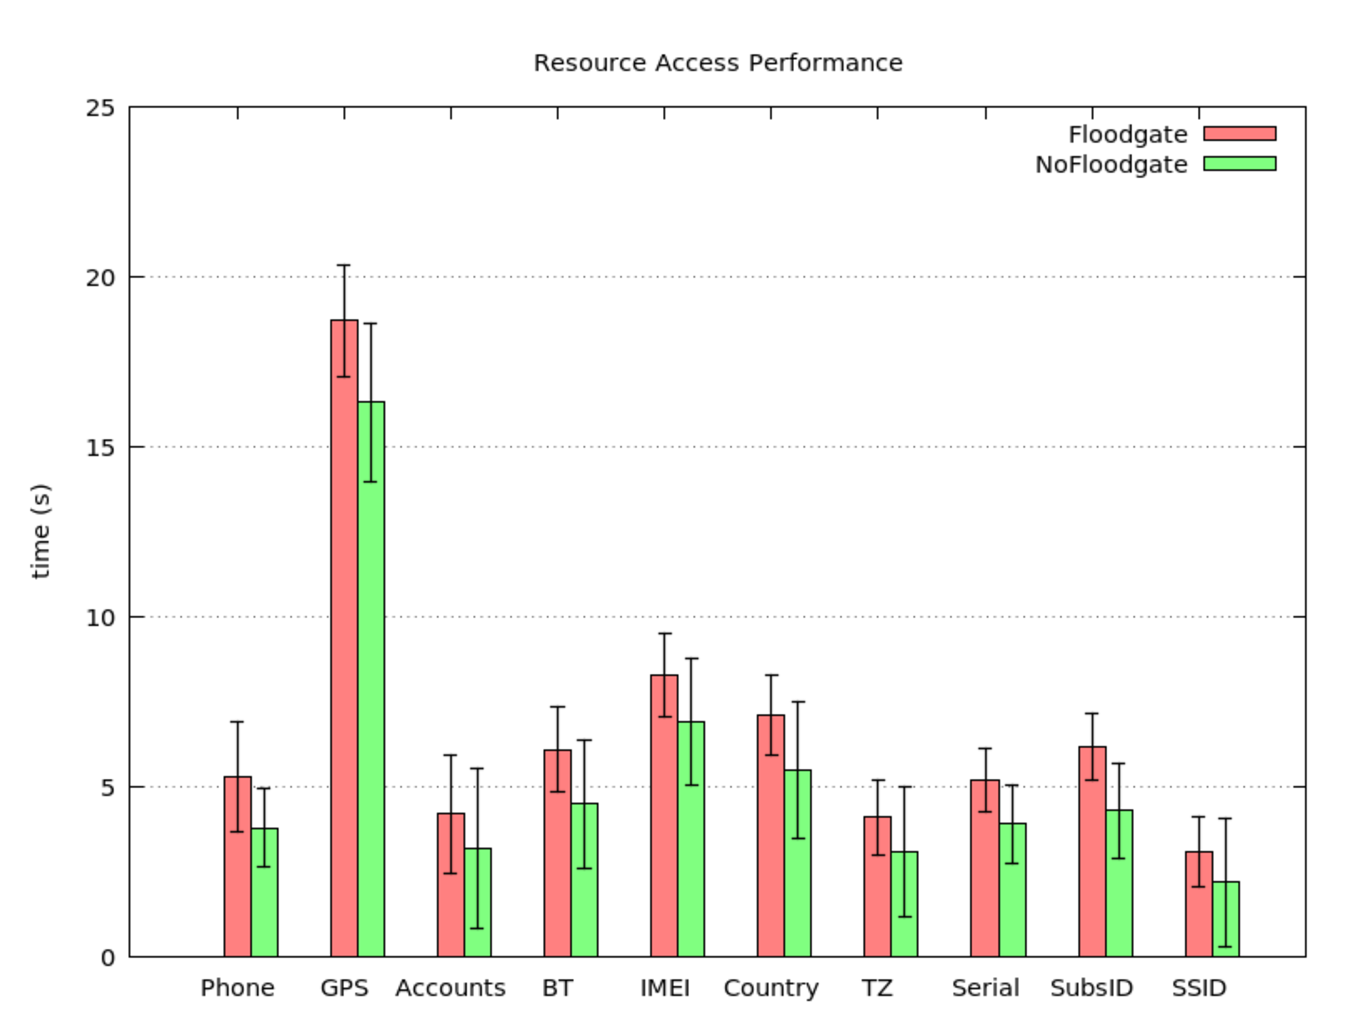
\includegraphics[width=\textwidth]{figs/mobile-performance}
\centering
\caption{Mobile-side performance impact}
\label{fig:mobile-performance}
\end{figure}

\section{Server-side Performance Impact}
\label{sec:server-performance}

Here we will present the test plan, results and respective discussion for evaluating Floodgate's impact on our backend.

To evaluate the impact of dealing with instrumented data and performing operations with this data on the server-side, we defined a metric to measure that impact: We chose the execution time and memory usage of server-side programs when in the presence of Floodgate. We focused our test plan on the DaCapo \footnote{\url{http://www.dacapobench.org/}} 9.12-bach macro-benchmark suite, which contains 14 benchmarks and simulates real-world applications within its workloads, manipulating multiple data types. All these benchmarks were ran using the \textit{``default''} size workload. We measured the execution time and maximum JVM heap usage. Due to the augmented number of instructions on the Floodgate-instrumented version of the programs, a substantial overhead was expected.
The test results are represented on Fig. \ref{fig:server-performance} and \ref{fig:server-memory}, for execution times and JVM heap usage, respectively.

\begin{figure}[t!]
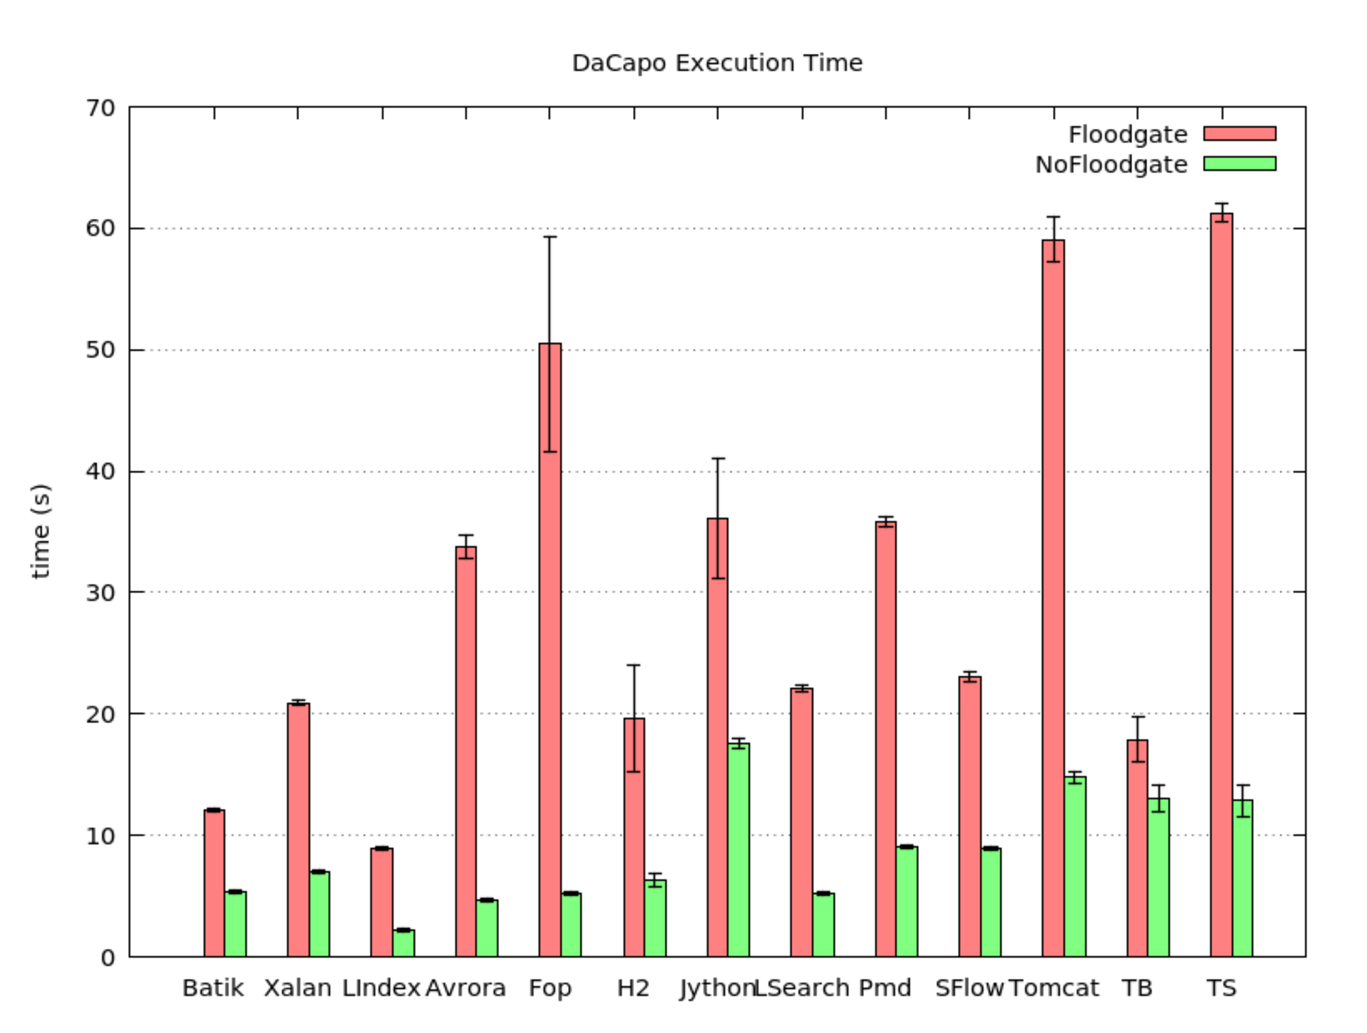
\includegraphics[width=\textwidth]{figs/server-performance}
\centering
\caption{Server-side performance impact}
\label{fig:server-performance}
\end{figure}

Analyzing the results, we spot that Floodgate introduces an overhead of about three times on the \textit{backend} performance. Despite it is a considerable value, each of the performed tests was specifically engineered to test different and heavy operations. Looking closely to Fig. \ref{fig:server-performance}, we can conclude that Floodgate behaves better in some of the tests than in others. Concretely, Floodgate introduced lower overhead values when executing the Batik or Xalan benchmarks. On the one side, the Batik benchmark consists in converting image files from \texttt{.png} to \texttt{.svg} format. The Xalan benchmark, on the other side, transforms XML into HTML documents. In opposition, the Fop or Avrora benchmarks introduced higher overhead values. Their execution consist in parsing an XSL-FO file and converting it to PDF, and simulating a number of programs running on a grid of AVR microcontrollers, respectively. In conclusion, Floodgate's \textit{backend} performance can prove itself better, depending on the kind of operations performed by the application at the server-side.

\begin{figure}[t!]
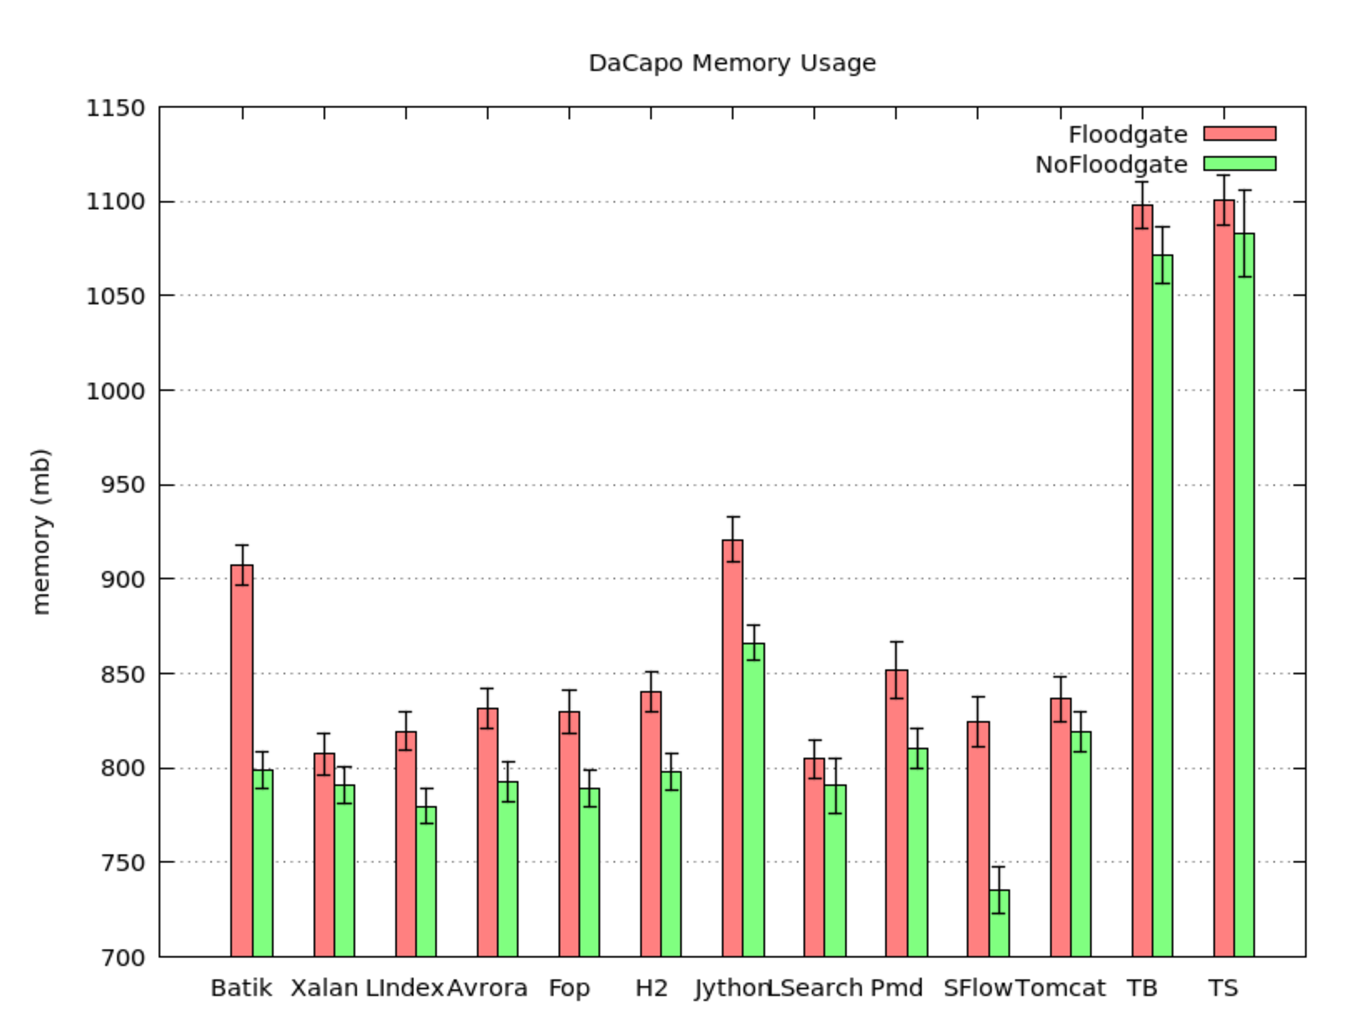
\includegraphics[width=\textwidth]{figs/server-memory}
\centering
\caption{Server-side memory usage impact}
\label{fig:server-memory}
\end{figure}

In contrast, the maximum memory heap usage test showed that Floodgate introduced an overhead of about 5.2\%, which we consider a great result. Since the performed tests were very resource-consuming, Floodgate server showed here some memory-usage efficiency.

\section{Mobile-server Interactions' Latency}
\label{sec:mobile-server-latency-eval}

Since Floodgate's target are \textit{backend}-supported mobile applications, which functionality rely on network requests made between mobile and server \textit{endpoints}, these requests' latency is also an important test metric to evaluate our system. These target mobile applications' functionality is often based on mobile \textit{endpoints} consuming resources (i.e. API methods) offered by a \textit{backend}. 

In this section, we will present a test plan, the respective results and critics, regarding the network requests' latency imposed by Floodgate during its operation.

So, to evaluate the request's latency imposed by Floodgate, we developed a simple application which works as a \textit{baseline} for test purposes. In the mobile endpoint, the application accesses the device's phone number and sends it through an HTTP request to the \textit{backend}. The \textit{backend}, by its turn, simply returns the same phone number, concatenated with the string ``ok!''. Finally, the mobile device prints the \texttt{<phone\_number> + ok!} message on the screen. 

Our test plan consisted in measuring the time spent by the three components we can spot here: The mobile endpoint, in which Floodgate controls the access to the phone number and generates the network request. The \textit{backend}, responsible for receiving the resource and generating the response. And the network, responsible for delivering the network request and returning the correspondent response. By comparing the Floodgate and the non-Floodgate versions, we expected increases in both the mobile-side and server-side components, due to Floodgate's operation, but similar measures in the network component. This is because all that Floodgate adds to the network requests is a ``privacy'' header, which we think is not a relevant addition in terms of time to deliver the requests.

The results for all the components' execution times are represented in Fig. \ref{fig:mobile-server-latency}.

\begin{figure}[t!]
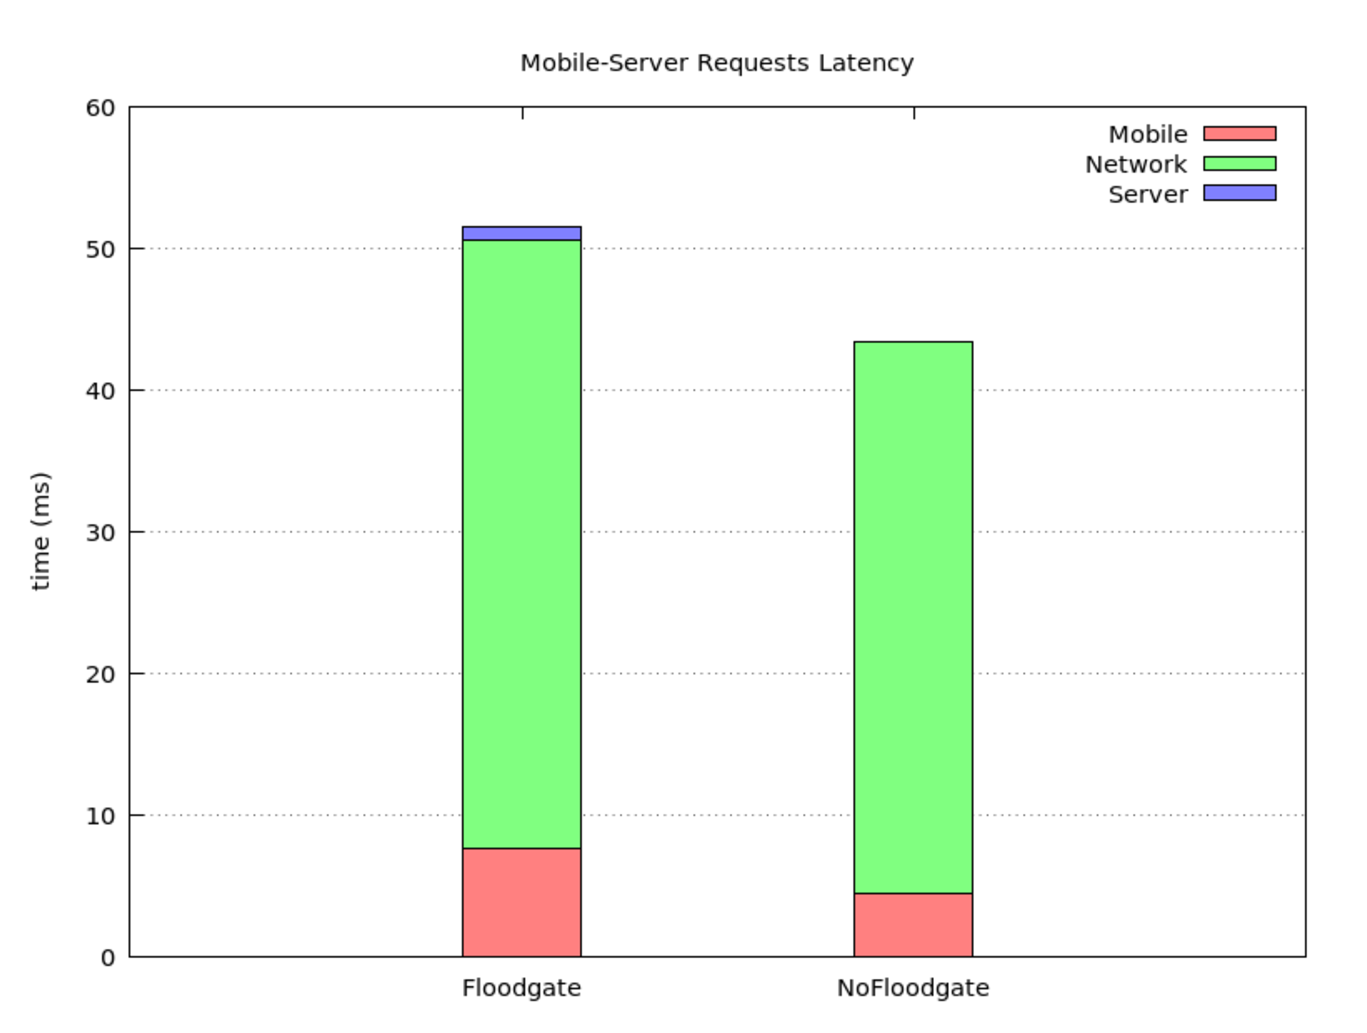
\includegraphics[width=\textwidth]{figs/mobile-server-latency}
\centering
\caption{Mobile-server latency}
\label{fig:mobile-server-latency}
\end{figure}

The results showed that Floodgate introduced an impact of about 69\% on the mobile-side performance, 10\% on the network component and also an overhead of about 400 times on the server-side performance.

On the mobile-side, the observed results somehow matched with the expected ones. In this test, we accessed the device's phone number and sent it through the network, measuring the execution time on the mobile-side only, just as we did on Sect. \ref{sec:mobile-performance} with multiple mobile resources. On that test, accessing the mobile phone number with Floodgate showed an overhead of about 40\%. Although, the test ended when the phone number privacy was added to the HTTP request's headers. In this test, the increased overhead may be justified in part by the time spent for the mobile device to process the HTTP response and present it on the mobile device's screen.

The network component, with an average overhead of 10\%, also makes us assuming it as a good result. Despite most Floodgate operation occurs both on the mobile and server-sides, we can justify the network overhead with the fact that, with Floodgate, each HTTP request will carry an additional HTTP header, the ``privacy''. Still, we consider that this result doesn't harm the practical user experience with Floodgate applications.

Finally, the server-side verified an excessive overhead of about 400 times. On Sect. \ref{sec:server-performance}, we already measured the server-side performance under heavy operations, which showed an overhead of about 300 times. Although, this time our \textit{backend} only executed a simple baseline operation of returning the input sent by the mobile device. Due to that, the execution times revealed themselves really small. The no-Floodgate version of the server spent an average of 0.0022 milliseconds to complete this task. Applying the Floodgate server instrumentation, this time increased to an average of 0.90 milliseconds. This way, we justify the giant overhead with the fact that it can easily occur when execution times are of these order of magnitude.

In conclusion, we consider these results as average ones, given that, in practice, we consider this doesn't prejudice the user experience with the application.

\section{Database Read/Write Operations Performance}

Another meaningful test plan we performed considered the performance of read/write operations of the \textit{backend} database, since all common application \textit{backends} have to persistently store their data. In this section, we will present the test plan and respective results that we prepared to test Floodgate applications' database performance. Floodgate, or concretely the Dropwizard framework, provides managed access to JDBI, a flexible and modular library for interacting with relational databases via SQL.

In this test plan, we took the simple application we created for the evaluation on \ref{sec:mobile-server-latency-eval} and created a simple database on our \textit{backend} that could handle the phone numbers arriving there. Also, we implemented a method on the mobile \textit{endpoint} application to query the database for the existing phone numbers. Here we measured the average time spent by Floodgate on two essential database operations: Writing a new phone number to the database; and reading the existing phone numbers, by querying the database.

\begin{figure}[t!]
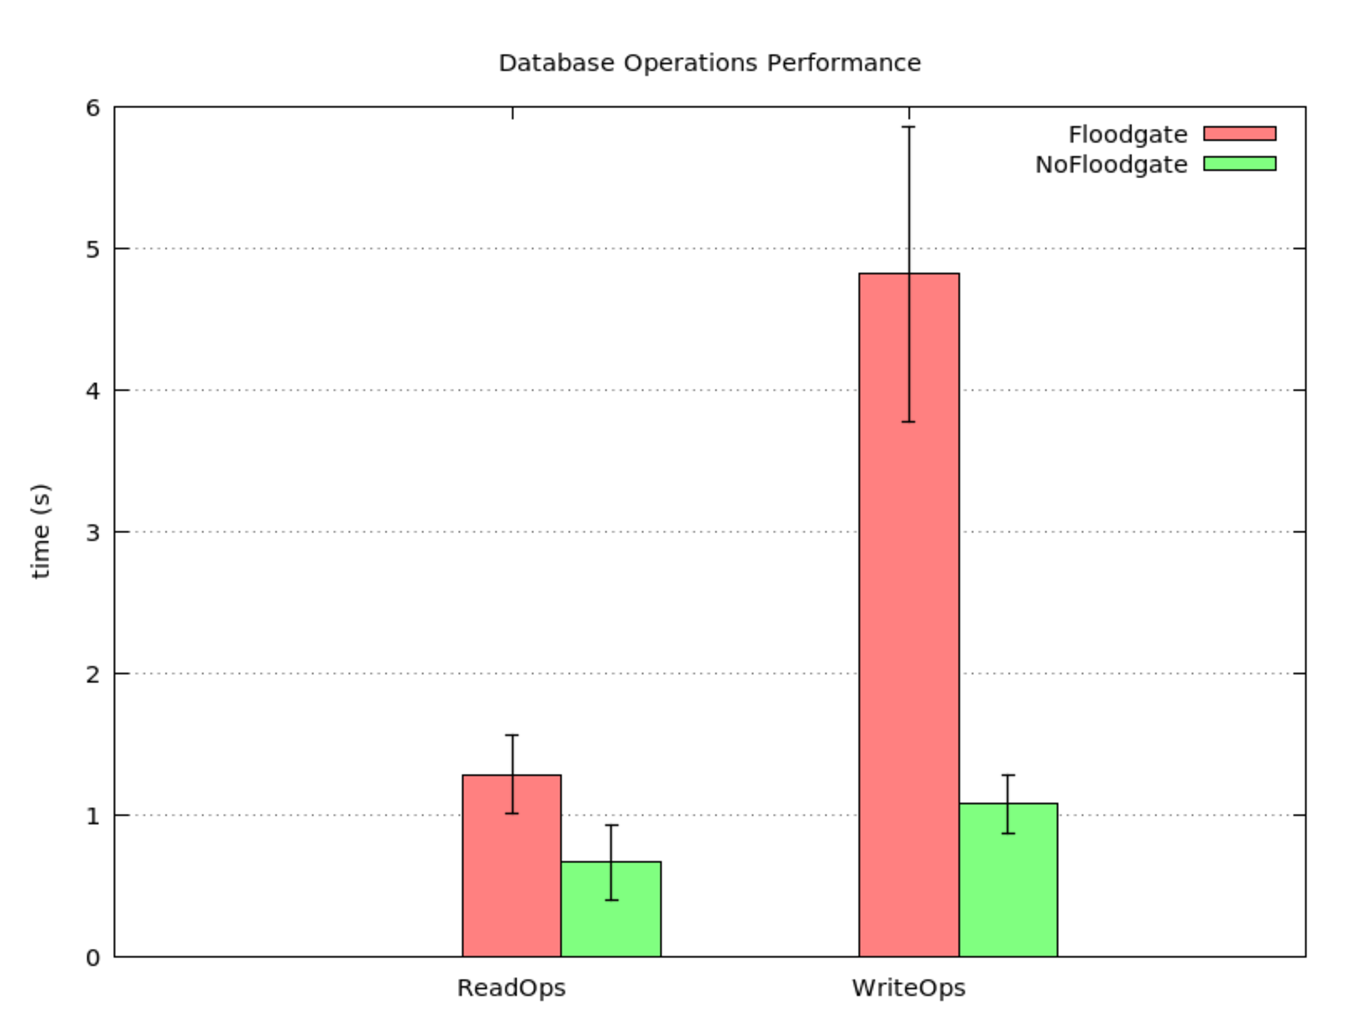
\includegraphics[width=\textwidth]{figs/database-performance}
\centering
\caption{Floodgate database performance}
\label{fig:database-performance}
\end{figure}

The results on Fig. \ref{fig:database-performance} show that Floodgate imposes an overhead of about 5.8 times when writing an object to the database, and an overhead of about 1.9 times when reading from the database.

During read operations, the verified results can be classified as extremely positive. This is because every time an object is read from the database on a Floodgate server, another query is automatically executed to our persistence taint module, in order to find the respective taint tag, and assign it to the object. This way, an overhead of 1.9 times matches the expected result. 

On the other side, write operations reveal a higher overhead (5.8 times). Just like in read operations, when an object is written to the database Floodgate provides, another object containing the first's taint tag must be written to the persistence taint database. So, we can conclude that Floodgate behaves worse during write operations, but the verified results somehow match the expected ones, since write operations to all common databases are more time-consuming, when compared to read operations.

\section{Use-case Application}

Apart from the quantitative evaluation we presented on above, Floodgate was also qualitatively evaluated. To do that, we developed an use-case application, with both mobile and \textit{backend} components, as near as possible to a real-world application which could at the same time provide a useful service to its users and show all the Floodgate's functionality. This way, we implemented AuctionsApp. As the name implies, it consists in an auctions app that allows users to post items for auctioning and live bidding on any available item except the ones they posted itself. 

To test Floodgate's operation, we developed a permissions manifest in which we declared the device's phone number as a private resource, and then we implemented an willful security flaw. For instance, every time a user puts a bid on any item, the mobile application will access the device's phone number, and send it through the network to the \textit{backend}, along with the bid's information. Here, Floodgate ensures that all the requests exchanged between the mobile and server sides will include the ``privacy'' header to state whether the request's content is tainted or not. 

On the server-side, the application receives the request and creates the bid, persistently storing the incoming information and updating the price of the item to which the bid applies. Also, Floodgate  filters the request, enforcing incoming taints to be applied to data, right before this data enters the \textit{backend's} application flow and enforces taints to be persistently stored at the same time as their correspondent data.

Every time a user asks for the list of current available items (whose auction periods haven't expired yet), it triggers an action on the Floodgate's server which can be decomposed on multiple parts: First of all, the application queries the persistent database for all the open auctions available. After that, Floodgate checks whether each one of these items have a correspondent persistent taints. If so, those taints are applied before the items leave the database and enter the application flow. After that, the application produces an HTTP response with the information of all available items and calls network methods to dispatch it. Although, this response will be filtered by the outcoming HTTP filters present on the \textit{backend}, in order to check whether the content being exported is, therefore, tainted. If it is, Floodgate is able to block the response or to let it proceed based on certain checks, to be defined by the programmer itself (i.e. destination endpoint, taint type, etc.).

\section{Security Evaluation}



    
 

%%%%%%%%%%%%%%%%%%%%%%%%%%%%%%%%%%%%%%%%%%%%%%%%%%%%%%%%%%%%%%%%%%%%%%%%%%%%%%%%%%%%%%%%%%%
%                               Conclusions - 2pp
%%%%%%%%%%%%%%%%%%%%%%%%%%%%%%%%%%%%%%%%%%%%%%%%%%%%%%%%%%%%%%%%%%%%%%%%%%%%%%%%%%%%%%%%%%%
\chapter{Conclusions}
\label{sec:conclusions}

\section{Conclusions}
We have described the design, implementation, and
experimental evaluation of  My System. Bla bla.

\section{Future Work}

As future work we would like bla bla.


\bibliographystyle{ieeetr}
\bibliography{references}
\addcontentsline{toc}{chapter}{{\small Bibliography}}


\end{document}
